%% need help with git?
%% http://www.desy.de/~bargheer/gitintro/git.html

\documentclass[parskip,bibtotoc,final,twoside=false,titlepage,a4paper,english,12pt,titlepage,a4paper]{scrbook}
% % twoside=true							makes sure new chapters start on rightside (even pagenumber)
% % BCOR10mm, DIV10					Binding Correction of 10mm (better 2cm?), shifts lower and upper
% % parskip 					Absatz mit Leerzeile
% % bibtotoc					Literaturverzeichnis in Inhaltsverzeichnis aufnehmen
% % listotoc 				Listen in Inhaltsverzeichnis aufnehmen
% % headsepline 			Trennlinie nach Kopfzeile
% % chapterprefix		"Chapter ##" steht in einer Zeile vor Chapter-Name
% % onelinecaption		falls einzeilige Überschrift bei Tab. Fig. dann zentriert
% % cleardoubleempty	leere Seite auch wirklich leer
% % DIV10, BCOR1cm 	Bindkorrektur

\pagestyle{plain}
\usepackage[utf8]{inputenc}
\usepackage[headsepline,footsepline,plainfootsepline,markcase=upper]{scrlayer-scrpage}
\usepackage{amsmath,amssymb}
\usepackage{graphicx}
\graphicspath{ {../fig/} }
\usepackage{caption}
\usepackage{subcaption}
\usepackage{cite}
\usepackage{copyrightbox}
\usepackage{booktabs}
\usepackage[colorlinks=false]{hyperref} %For creating hyperlinks in cross references
\usepackage[onehalfspacing]{setspace}
\usepackage{enumitem}
\setlist{nosep}

% \usepackage[%
%   backend=bibtex      % biber or bibtex
% %,style=authoryear    % Alphabeticalsch
%  ,style=numeric-comp  % numerical-compressed
%  ,sorting=none        % no sorting
%  ,sortcites=true      % some other example options ...
%  ,block=none
%  ,indexing=false
%  ,citereset=none
%  ,isbn=true
%  ,url=true
%  ,doi=true            % prints doi
%  ,natbib=true         % if you need natbib functions
% ]{biblatex}

\makeindex

\title{Bachelor Thesis:\\
“Software implementation of the quality assurance tool for magnetic resonance imaging distortion assessment”}
\author{David Blacher}
\date{DRAFT \today }

\renewcommand*{\chapterheadstartvskip}{\vspace*{-\baselineskip}}
\renewcommand*{\chapterheadendvskip}{\vspace*{0cm}}
% http://tex.stackexchange.com/questions/130260/koma-script-scrbook-how-to-change-v-space-between-chapter-prefix-and-title

\begin{document}
\pagenumbering{arabic}
\maketitle
\tableofcontents
\cleardoublepage

%\section{Acknowledgements}

%\listoffigures
%\listoftables

%\section{Abbreviations}

% Purpose, Materials and Methods, Results, Conclusion

\chapter*{Abstract}
Purpose, Materials and Methods, Results, Conclusion



\chapter{Introduction}
% o General: Start with very general description and focus step by step on your topic
% o keep in mind, that the introduction usually contains the most references
% o Introduction to main topic (e.g. Radiotherapy, MRI, ...) including historical review (1-2pages), Purpose of Radiotherapy ; Regardless of your actual topic, put it in context to conventional photon radiotherapy
% o Basic principles of Physics related to your topic
% o (e.g. Photo effect, Compton effect, Bethe-Bloch equation, ...)
% o Technological Background related to your topic
% o Give a general descriptions about the devices used in your thesis
% o (e.g. Linac, Afterloader, Synchrotron, Detectors...)
% o Overview of literature connected to your topic
% o Purpose of the thesis
% o based on the literature research, describe which information is missing, describe briefly what your thesis is about and what is the novelty of your work

\section{Types of External Beam Radiation Therapy}
External Beam Radiation Therapy (EBRT) utilizes ionizing radiation to damage cancer cells in order to stop them from multiplying.
This prevents the growth of tumours and eventually cures the patient. 
In conventional EBRT photons (x-rays) in the range of 4MeV to 20MeV are used to administer the necessary dose at the location of the tumour. Unfortunately, photons interact with all cells
they're passing through until they are fully stopped. They release their energy slowly while travelling through the patient and usually get completely absorbed after leaving the body.
Charged particles (e.g. protons, carbon ions) minimize the damage done to healthy tissue due to their distinctive behaviour in energy loss called ``Bragg Peak''.
They release most of their energy shortly before stopping. \cite{Nakamura2010} This effect can be used to spare tissue lying behind the tumour from radiation. \cite{Paganetti2005} % and before
A comparison between x-rays and protons is shown in figure \ref{fig:bragg}.

\begin{figure}[!h]
\centering
\copyrightbox{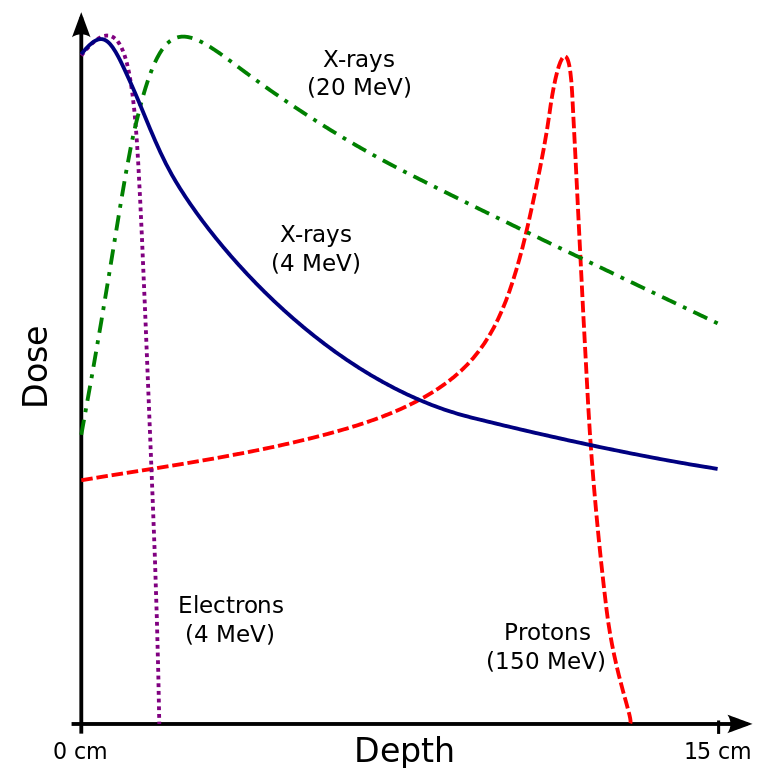
\includegraphics[width=0.6\textwidth]{Dose_Depth_Curves.png}}{\vspace{1cm}By Cepheiden,\\ GFDL ($http://www.gnu.org/copyleft/fdl.html$), via Wikimedia Commons}
\caption{energy release of ionizing radiation}
\label{fig:bragg}
\end{figure}

While travelling through matter both types of radiation release energy mostly due to coulomb interactions with the outer shell electrons of atoms.
Knowing the electron density of of the targeted tissue area is therefore essential. In order to reach a specific penetration depth, the particles' initial energy has to be chosen accordingly.

\section{Role of CT}

Until recently radiotherapy treatment planning (RTTP) relied heavily on Computer Tomography (CT). There are two main reasons for this:

Firstly, CT uses low energy x-rays to create a 3D image of the patient. The luminosity value (brightness) assigned to each voxel (like pixel, but three-dimensional) corresponds to
the local radiodensity recorded in Hounsfield units ($HU$). Materials with a higher radiodensity (e.g. bones) absorb more x-ray photons than those with less (e.g. water, brain-mater).
Calculating the electron density using data obtained with CT is an easy task and used widely for RTTP. \cite{Constantinou2012, Schneider1996}
In order not to induce new cancer cells in healthy tissue during EBRT, the radiation beams are carefully targeted using the measured radiodensity. 
This way the absorbed dose accumulates in the cancer regions, while the nearby healthy tissue receives less radiation.

Secondly, CT images generate 3D images with little distortion. Exact geometries are needed for correct RTTP. %more details

\vspace{4cm}
\textit{Image of RTTP}
\vspace{2cm}

\section{Role of MRI}

% mri needs coils
% mri can create differently weighted images (T1, T2, etc..)


Today RTTP often combines CT images with data acquired using Magnetic Resonance Imaging (MRI).
MRI scans also record luminosity values, but they do not correspond to $HU$ (radiodensity measured by CT).
The signal intensity depends on many factors and even varies between MRI scanners.

MRI uses strong stationary magnetic fields to align magnetic spin moments of protons. Then an additional alternating field resonating with the spins is applied shortly to flip them $90^o$.
Depending on the material spins then take longer or shorter to align again with the stationary field. Those differences can be measured in a pick-up coil surrounding the
region of interest. The nature of this effect leads to a great contrast between soft tissue. \cite{Currie2013} Delineating tumours using MRI images is more accurate than using CT.
\cite{Rasch1999, Debois1999a, Roach1996}

Another advantage of MRI over CT is the harmlessness of magnetic fields. CT utilizes the same type of radiation used for destroying cancer cells. Even though the radiation dose of a
CT is low compared to radiation therapy, cancer patients need to be imaged frequently during treatment planning. Especially children treated with EBRT typically
suffer from induced cancer occurring up to 40 years later. So while the benefit from using CT for diagnostics far outweighs the damage, there have been major efforts to
reduce dose while maintaining reasonable image quality. \cite{Murphy2007, Brenner2001, Sodickson2009, Smith2007, McCollough2009, Goldman2013}

There are some difficulties arising from combining CT and MRI for EBRT:
In order to profit from separately acquired data, the resulting images must be aligned either manually or automatically. This is a hard task since non-rigid objects (organs) change their shape and location between measurements. This leads to inaccuracies.
Therefore MRI-only radiation therapy protocols are being developed:
MRI data is used to create a Pseudo-CT, which contains information about electron density. Comparisons to using CT and MRI have shown acceptable deviations for X-ray therapy.
In charged particle therapy the resulting dose gain in healthy tissue and dose loss in cancer regions due to inaccurately assigned electron density values is bigger.
However, current development is promising. \cite{Rank2013, Stanescu2006, Nyholm2015, Greer2015, Chen2004}

\section{Open bore MRI scanners}

% advantages of low tesla, brachytherapy
The radiation oncology department of the Vienna General Hospital (AKH) is equipped with an 0.35T open-bore, c-arm MRI scanner. The open design improves the well-being of patients
experiencing anxiety in closed scanners. Consequently, the number of incomplete MR examinations due to a claustrophobic events is low. \cite{Enders2011a, Bangard2007}
Besides, patients who wouldn't fit in closed designed scanners can be imaged.
Also, brachytherapy patients can be placed in the scanner with applicators attached.

This type of scanner is weaker than a conventional closed bore scanner (1-3 Tesla). High field strengths would result in greater resolution, better Signal to Noise (SNR) ratio, and faster imaging time.
However, ``There are definite cost advantages (capital, operating, siting) to the use of lower field MRI.'' \cite{Rutt1996}
% capital, operating, siting????
Permanent magnets are sufficient to create the 0.35T field. Therefore there is no need for constant cooling using liquid helium compared to superconducting magnets.
Consequently, maintenance and service costs are considerably lower.

Generally, diagnostics benefit from greater image quality. However, at some point diagnostic accuracy stops increasing with field strength.
Nevertheless, high field scanners are key to developing new methods such as functional MRI (fMRI) of the brain \cite{Duyn2012} and observing
``metabolic reactions occurring in a human body in addition to producing very precise images of body structures'' \cite{Wada2010}.
At the same time astonishing improvements can be achieved at low fields.
A ``combination of field independent polarization [...] with frequency optimized MRI detection coils [...] results in low-field MRI sensitivity approaching and even rivaling that of high-field MRI.'' \cite{Coffey2013}

One drawback of MRI, and especially open bore scanners, is the occuring distortion due to inhomogeneities in the magnetic field.
For most applications small position shifts and deformations are of minor importance. In RTTP however, those effects can have a big impact.
Therefore MRI scanners usually come equipped with an internal distortion correction algorithm.
Those methods are developed by the company designing the scanners. Knowing the technical details enables them to drastically reduce the distortion.

Field of view (FOV) of the MRI scanner is smaller than the CT scanner's.

\section{Aim of this work}
The used open bore MRI scanner is not intended to be used for RTTP. The on board correction algorithm might not be good enough for effetive EBRT.
The goal of this work is to commence the development of a quality assurance tool to asses the spatial distortion (after applying the internal correction).
This is achieved by comparing MRI images to CT images used as a gold standard.
An alerady existing custom designed phantom is provided by the AKH Vienna for this purpose.
However, the liquid to fill the rods with has not been chosen yet.
Therefore, this paper focuses mainly on the acquired data and which liquids to use the phantom with, not its entire design.
However, possible fillings have to be produced and tested.
Similar approaches are being used for distortion correction by other facilities. \cite{Price2015, Petersch2004, Torfeh2015, Wang2004, Wang2004b, Mizowaki2000}

\chapter{Material and methods}

%  Everything that is mentioned in results, has to be mentioned here
%  Everybody who reads thesis, must be able to reproduce the experiment/study
% o Describe all materials, devices and methods, which were used in your work
% o if you describe a device, start with the brand name followed by the company name, city and country in parentheses: e.g. "... a VersaHD (Elekta AB, Stockholm, Sweden) was used in ...".
% o Provide some information on each device
%  e.g Linac, which energies were used, what was the field size, what was the leaf width, how is the linac calibrated, ...;
%  e.g. Detector array: which type of detector, how many detectors, what is the resolution, energy dependence, linearity,...;
%  e.g. Panning systems: software version, algorithms, settings used in this study
%  e.g. software: version, functionality
% o Also describe used data (patient cohort) even if they were taken from other studies

\section{Scanners}

CT and MRI scanners used during this work are listed in Table \ref{tab:scanners}.

\begin{table}[h]
\centering
\begin{tabular}{llll}
System	& product name	& company	& coil [internal W x H]		\\
\toprule
MRI	& Magnetom C!	& Siemens	& Body/Spine Array Coil XL	\\
	&		&		& [50 x 30.5 cm (19.7 x 12 in)]	\\
CT	&		&		& --------
\end{tabular}
\caption{used scanners}
\label{tab:scanners}
\end{table}

\section{Custom build phantom}

To measure distortion the scanners must image a rigid object with known dimensions.
Such phantoms are commercially available, but often expensive and designed for a specific calibration protocol.
Some institutions build their own to fullfill exactly the requirements of a given application.

For the AKH it was important to create a lightweight phantom which can be imaged by CT and MRI scanners.
Due to the underlying physics, only fluids are visible in MRI scans. CT however, also shows plastic.
See figure \ref{fig:sagittal_comparison} for a comparison (MRI/CT visibility).
Therefore, they decided on plastic rods with a suitable fluid filling.
Such a liquid should be easily produced, non-toxic, and yielding sufficient signal in MRI scans.

Commercially available phantoms often resemble water filled tanks containing plastic grids as a reference.
This design results in stronger signal, but exceeds practical weight.
There are few brands offering solutions utilising liquid fiducial markers in the shape of pellets.
They are arranged in a regular pattern surrounded by air or plastic.
The AKH's design however relies on replaceable rods, which makes it a novelty.


\begin{figure}[!htb]
\centering
  \begin{subfigure}[b]{0.1\textwidth}
    
\includegraphics[scale=1]{slicer3D/full_phantom/sagittal_comparison_mr.png}
    \caption{MR}
    \label{fig:sagittal_comparison_mr}
  \end{subfigure}
  \begin{subfigure}[b]{0.1\textwidth}
    
\includegraphics[scale=1]{slicer3D/full_phantom/sagittal_comparison_ct_empty.png}
    \caption{CT}
    \label{fig:sagittal_comparison_ct_empty}
  \end{subfigure}
  \begin{subfigure}[b]{0.1\textwidth}
    
\includegraphics[scale=1]{slicer3D/full_phantom/sagittal_comparison_ct.png}
    \caption{CT}
    \label{fig:sagittal_comparison_ct}
  \end{subfigure}
  \caption{Comparison: MRI only shows liquid filling, CT also the plastic rod and pane (horizontal black bar crossing middle and right rod);\\ (\textbf{a:}) \textit{MRI} - filled rod, plastic not visible (field of view too small to show entire rod); (\textbf{b:}) \textit{CT} - empty rod, plastic visible; (\textbf{c:}) \textit{CT} - filled rod, plastic and filling visible}
  \label{fig:sagittal_comparison}
\end{figure}

\subsection{Frame and rods}

For the open-bore MRI scanner the phantom was build to fit exactly the scanner's coil.
Three parallel acrylic glass panes in the shape of the coil serve as a rigid frame.
In the middle an empty area was reserved for an optional additional smaller phantom (not used for this work).
Figure \ref{fig:phantom_photo} shows an picture of the phantom. See also figure \ref{fig:axial_CT_pane} showing a CT image of one pane (with no rods inserted). \\
More than 300 plastic rods (length: 50cm, outer diameter: 8mm, inner diameter: 4mm, volume: approx. 6mL) could be placed in the phantom.
See figure \ref{fig:rod_schematic} for a schematic sketch.
The bottom part of each rod was sealed with a hot glued plastic plug, the top could be closed with a plastic screw.
Frame and rods were already build and assembled before the author started working on this project.


% photo of phantom

\begin{figure}[!tbp]
\centering
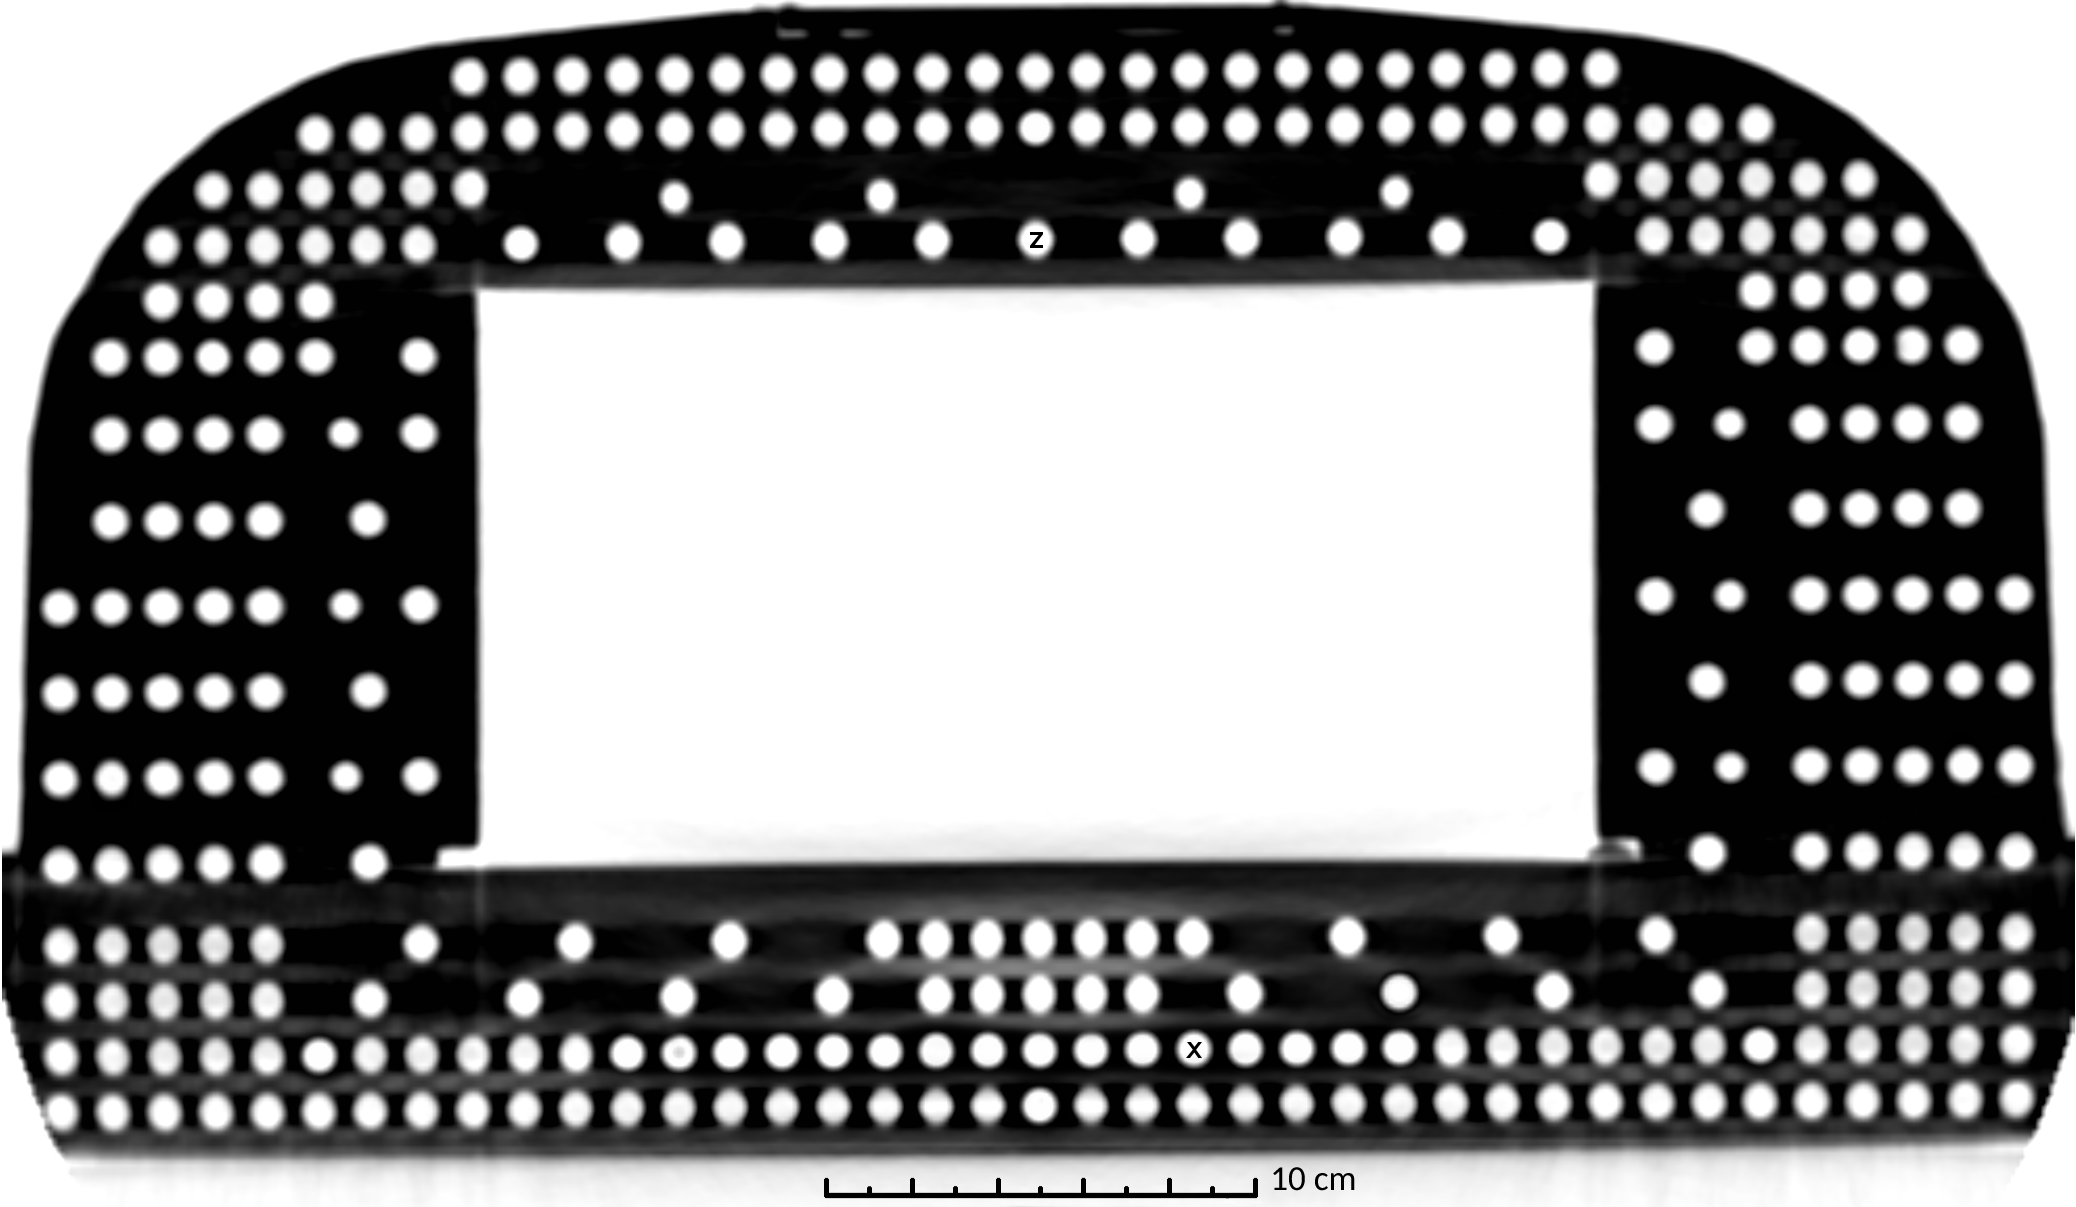
\includegraphics[width=\textwidth]{slicer3D/full_phantom/axial_CT_pane.png}
\caption{plastic pane, no rods inserted}
\label{fig:axial_CT_pane}
\end{figure}

\begin{figure}[!tbp]
\centering
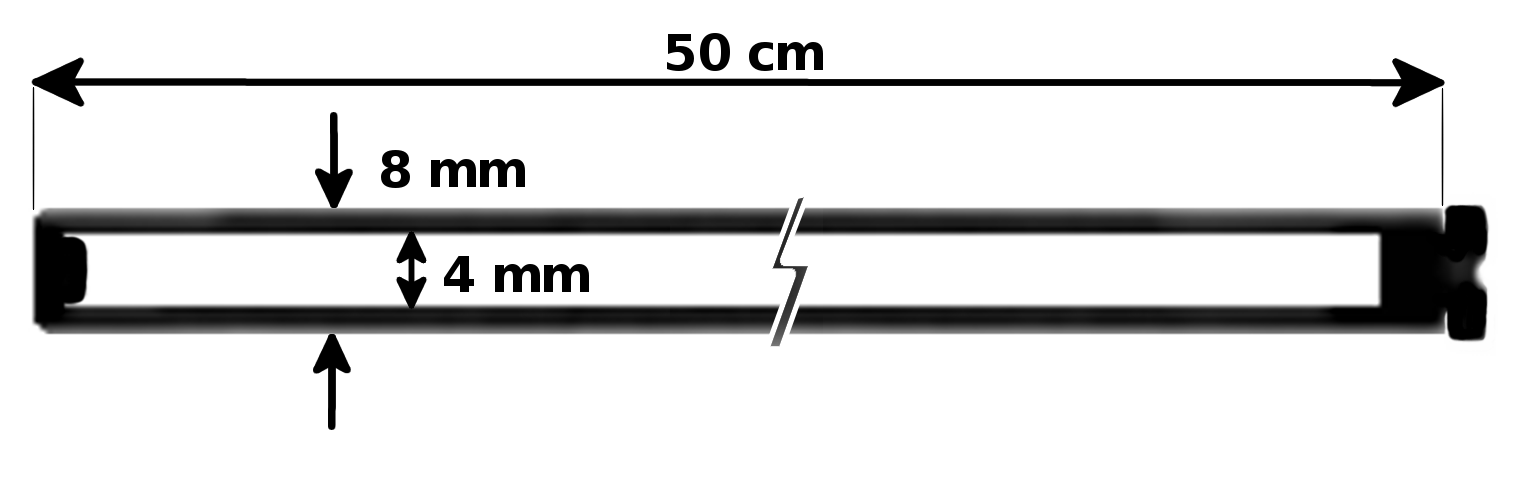
\includegraphics[width=0.8\textwidth]{slicer3D/full_phantom/rod_schematic.png}
\caption{empty plastic rod, schematic (not true proportions); }
\label{fig:rod_schematic}
\end{figure}

\vspace{4cm}
\textit{photo of Phantom}
\vspace{2cm}
\vspace{4cm}
\textit{photo of single rod}
\vspace{2cm}

\subsection{Rod fillings}

For this study 17 different liquids were produced to be tested as possible fillings. They are listed in Table \ref{tab:solutions}.

Most tested fluids are based on water. This makes it easy to empty and clean the rods if needed. They could then be filled again with a different liquid.
The chosen components are either non-toxic or harmless if not swallowed.
Unfortunately the water might evaporate over time. To improve the mobility of trapped air bubbles, soap was added to some fluids.

As an alternative 2 oils were proposed. They do not contain water and air is not soluble in oil. Once a rod is completely with oil, no air bubbles should form.
Using vegetable oil would be a non-toxic solution. This has been ruled out as a filling, because it would eventually rot.
Mineral oil on the other hand does not rot.


\begin{table}[!hbt]
\centering
\begin{tabular}{@{}l|rrrrrr@{}}
Nr.   & $NaCl$   & $CuSO_4\cdot5H_2O$          & Soap & Ascorbic Acid & Agar & Primovist [volume-\%]\\
\toprule
\#1  &             &                   &      &               &           &		\\
\#2  & 3.6         & 1.96              &      &               &           &		\\
\#3  & 3.6         & 3.92              &      &               &           &		\\
\#4  & 3.6         & 19.6              &      &               &           &		\\
\#5  & 3.6         & 1.96              & 1    &               &           &		\\
\#6  & 3.6         & 1.96              & 5    &               &           &		\\
\#7  & 3.6         & 1.96              & 20   &               &           &		\\
\#8  & 3.6         & 1.96              &      & 0.36          &           &		\\
\#9  & 3.6         & 1.96              &      & 3.6           &           &		\\
\#10 & 3.6         & 1.96              &      & 36            &           &		\\
\#11 & 3.6         &                   &      &               &           & 0.1\%	\\
\#12 & 3.6         &                   &      &               &           & 1\%		\\
\#13 & 3.6         &                   &      &               &           & 10\%	\\
\#14 & 3.6         & 1.96              &      &               &  0.5      &		\\
\#15 & 3.6         & 1.96              &      &               &   20      &		\\
\midrule
\#16 & \multicolumn{2}{r}{Motor Oil:}   & \multicolumn{4}{l}{\textit{Castrol Power1}}      \\
\#17 & \multicolumn{2}{r}{Silicon Oil:} & \multicolumn{4}{l}{\textit{Charge: 15HLVY023}}   \\ \bottomrule
\end{tabular}
\caption{composition of tested solutions\\(components in $g/L$; exception: Primovist in volume\%)}
\label{tab:solutions}
\end{table}

\newpage
\begin{enumerate}[label=\textbf{\#\arabic*}]
 \item \textit{destilled water} (as reference)
 \item $NaCl$ + $CuSO_4\cdot5H_2O$ (as suggested by AAPM MR Subcommittee \cite{Jackson2009})
 \item increased concentration of $CuSO_4\cdot5H_2O$
 \item further increased concentration of $CuSO_4\cdot5H_2O$
 \item generic washing-up \textit{soap} added to \textbf{\#2} (suggestion by Data Spectrum Corporation \cite{bubbles} to keep air bubbles from sticking to phantom walls)
 \item increased \textit{soap} concentration
 \item further increased \textit{soap} concentration
 \item \textit{ascorbic acid} added to \textbf{\#2} (reduce forming of air bubbles by binding dissolved oxygen. It then degrades to dehydro-ascorbic acid and water.
  \cite{Abtahi2008, Bodannes1979} Concentration of $0.36 \; g/L$ corresponds to approx. $0.00204 \; mol/L$)
 \item increased \textit{ascorbic acid} concentration
 \item further increased \textit{ascorbic acid} concentration
 \item \textit{Primovist} (a common contrast agent used for MRI scans \cite{VanBeers2012, Rohrer, primovist})
 \item increased amount of \textit{Primovist}
 \item further increased amount of \textit{Primovist}
 \item \textit{agar} (or agarose is commonly used as basic reference material for MRI phantoms \cite{BuccioliniCiraolo1989, Mathur-DeVre1985})
 \item increased \textit{agar} concentration
 \item synthetic motor oil
 \item silicon Oil
\end{enumerate}

% why those solutions??

Being closed at one end and having a capillary shape (small diameter) makes it impossible for the rods to be filled by pouring in the liquid.
Instead of adding the fluid at the top, it has to be injected starting at the bottom.
This way the contained air would pushed out through the opening on the top.
A thin plastic tube was used to leave room for the gas to escape.
Between different liquids the tube was flushed with \textbf{\#1} (destilled water) or \textbf{\#2} (main component of most solutions).

In order to minimize the amount of gas dissolved, the liquids were brought to boil shortly before injecting. Gas solubility generally decreases with rising temperature \cite{Henry1803, Sander2015}
After injecting the solution in the rods, they were left to cool down. Before closing the rods were topped up completely (no trapped air bubbles).
The oil based liquids, \textbf{\#16} and \textbf{\#17}, were not brought to boil.
Number \textbf{\#14} could be injected without problems, the solution remained fluid even after reaching room temperature.
Number \textbf{\#15} on the other hand changed to a gel like conistence and clogged the tube right after the rod was filled. The tube could not be used again.



\section{Sequences}

Following the suggestions given in the Report of AAPM MR Subcommittee TG1 ``MR Acceptance Testing and
Quality Control'' \cite{Jackson2009}, T1 weighted sequences were chosen to evaluate the possible solutions. (Table \ref{tab:settings})

\begin{table}[h]
\centering
\begin{tabular}{@{}lllll@{}}
System & ---  & --- &  --- & --- \\
\toprule
MRI    & -   & -   & -   & -    \\
CT     & -   & -   & -   &
\end{tabular}
\caption{used sequences}
\label{tab:settings}
\end{table}

\section{Developed software tool}

In order to asses the distortion of the MRI scanner, a tool was programmed.
It is written in Python 2.7 and uses the \textit{SimpleITK} package to read and process \textit{DICOM} (``\textit{Digital Imaging and Communications in Medicine}'') files. \cite{Python, DICOM}
\textit{SimpleITK} is a object-oriented ``C++ library with wrappers for Python, Java, CSharp, R, Tcl and Ruby''. \cite{SimpleITK, SimpleITK_started} It's versatility is one of the reasons why this approach was favoured.
It is a simplified layer built on top of the National Library of Medicine Insight Segmentation and Registration Toolkit (ITK). SimpleITK is also used by Applications like \textit{3D Slicer} , a ``free and open source software package for
visualization and medical image computing''. \cite{3DSlicer, Kikinis2012} For this work 3D Slicer was used to crop images, quickly read values and visualize the results.
Documentation and code examples of SimpleITK can be found at \cite{InsightSoftwareConsortium, Kyriakou-SimpleITK}
An alternative way to handle DICOM data in Python would be Pydicom. \cite{Pydicom, Kyriakou-Pydicom-VTK} 

An extensive list of packages used to process data:
\begin{itemize}
 \item SimpleITK
 \item numpy
 \item scipy
 \item matplotlib.pyplot \cite{Hunter2007}
 \item skimage.draw
 \item datetime
 \item os
\end{itemize}

\subsection{Processing MRI and CT scans}

% what application used to align CT and MRI
Prior to analising their data, the scans had to be prepared.
To start with, they were aligned in a way that yields maximum overlap especially in the centre of the image.
However, the MRI image had a lower resolution than the CT scan.
Therefore, the MRI voxel's size were changed to match the CT voxels. Both images were resampled to CT resolution.
Those steps were performed using \textit{MIRADA} (?????).

As described later, resolution might influence the efficiency of the distortion assesment.
The application \textit{3D Slicer} (Version: Slicer-4.5.0-1-linux-amd64) was used to again resample both images to a finer resolution.

Pixel spacing in x and y direction are equal. The z-axis, which lies approximately parallel to the phantom's rods, has a different pixel spacing.
Overall image resolution could have a significant effect on the results. Therefore all calculations were made using original and interpolated (increased resolution) scans.
See table \ref{tab:spacing} for more details. Figure \ref{fig:resample} depicts 3 CT/MRI scans of a single rod (axial) with different resolutions.
``x1'' stands for the original CT scan resolution (MRI resampled to match).
``x9'' is a resolution resulting in 1 pixel being splitted in 9 smaller pixels, ``x100'' in 100, and so on.
For better visibility images are printed with inverted colors. Dark pixels have a high density/intensity value, white pixels are equivalent to air (low density/intensity).

\begin{table}[!htb]
\centering
\begin{tabular}{l|l|l|l}
resample factor  & z (not affected) &  y (same as x) & x \\
\toprule
x1     & 0.600006 & 0.976563	& 0.976563	\\
x4     & 0.600006 & 0.488281	& 0.488281	\\
x9     & 0.600006 & 0.325521	& 0.325521	\\
% x16    & 0.600006 & 0.244141	& 0.244141	\\
x25    & 0.600006 & 0.195313	& 0.195313	\\
x100   & 0.600006 & 0.097656	& 0.097656
\end{tabular}
\caption{pixel Spacing [$mm$]}
\label{tab:spacing}
\end{table}


\begin{figure}[!thb]
  \begin{subfigure}[b]{0.32\textwidth}
    
\includegraphics[scale=.11]{slicer3D/profiles/CT_x1.png}
    \caption{CT x1}
    \label{fig:CT_x1}
  \end{subfigure}
  \hfill
  \begin{subfigure}[b]{0.32\textwidth}
    
\includegraphics[scale=.11]{slicer3D/profiles/CT_x9.png}
    \caption{CT x9}
    \label{fig:CT_x9}
  \end{subfigure}
    \hfill
  \begin{subfigure}[b]{0.32\textwidth}
    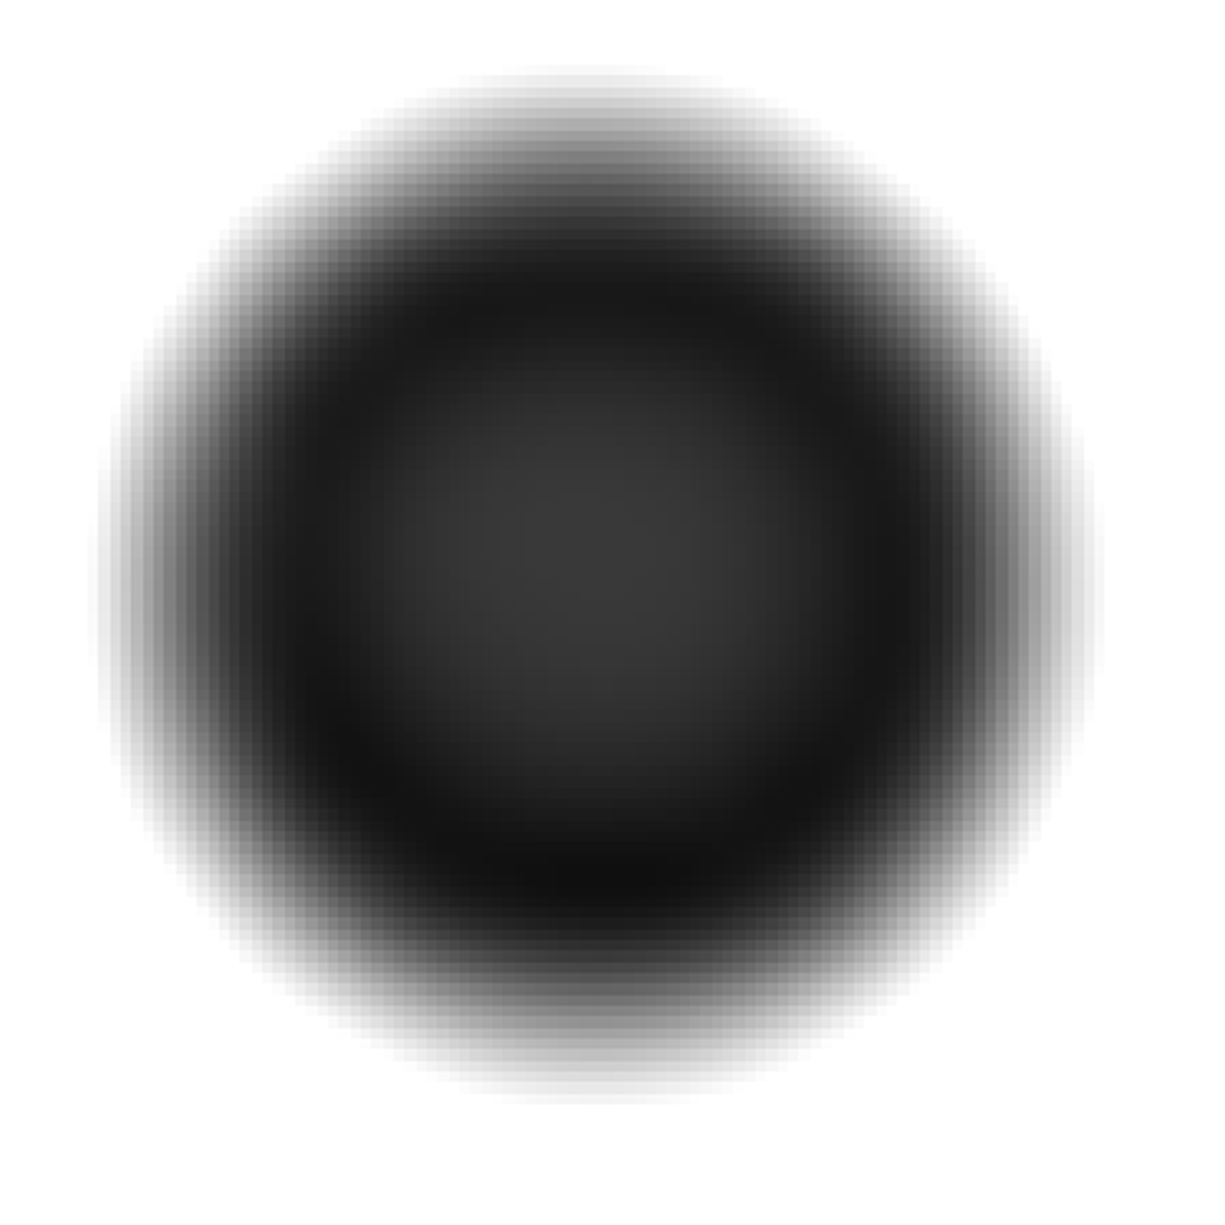
\includegraphics[scale=.11]{slicer3D/profiles/CT_x100.png}
    \caption{CT x100}
    \label{fig:CT_x100}
  \end{subfigure}
  \begin{subfigure}[b]{0.32\textwidth}
    
\includegraphics[scale=.11]{slicer3D/profiles/MR_x1.png}
    \caption{MRI x1}
    \label{fig:MRI_x1}
  \end{subfigure}
  \hfill
  \begin{subfigure}[b]{0.32\textwidth}
    
\includegraphics[scale=.11]{slicer3D/profiles/MR_x9.png}
    \caption{MRI x9}
    \label{fig:MRI_x9}
  \end{subfigure}
    \hfill
  \begin{subfigure}[b]{0.32\textwidth}
    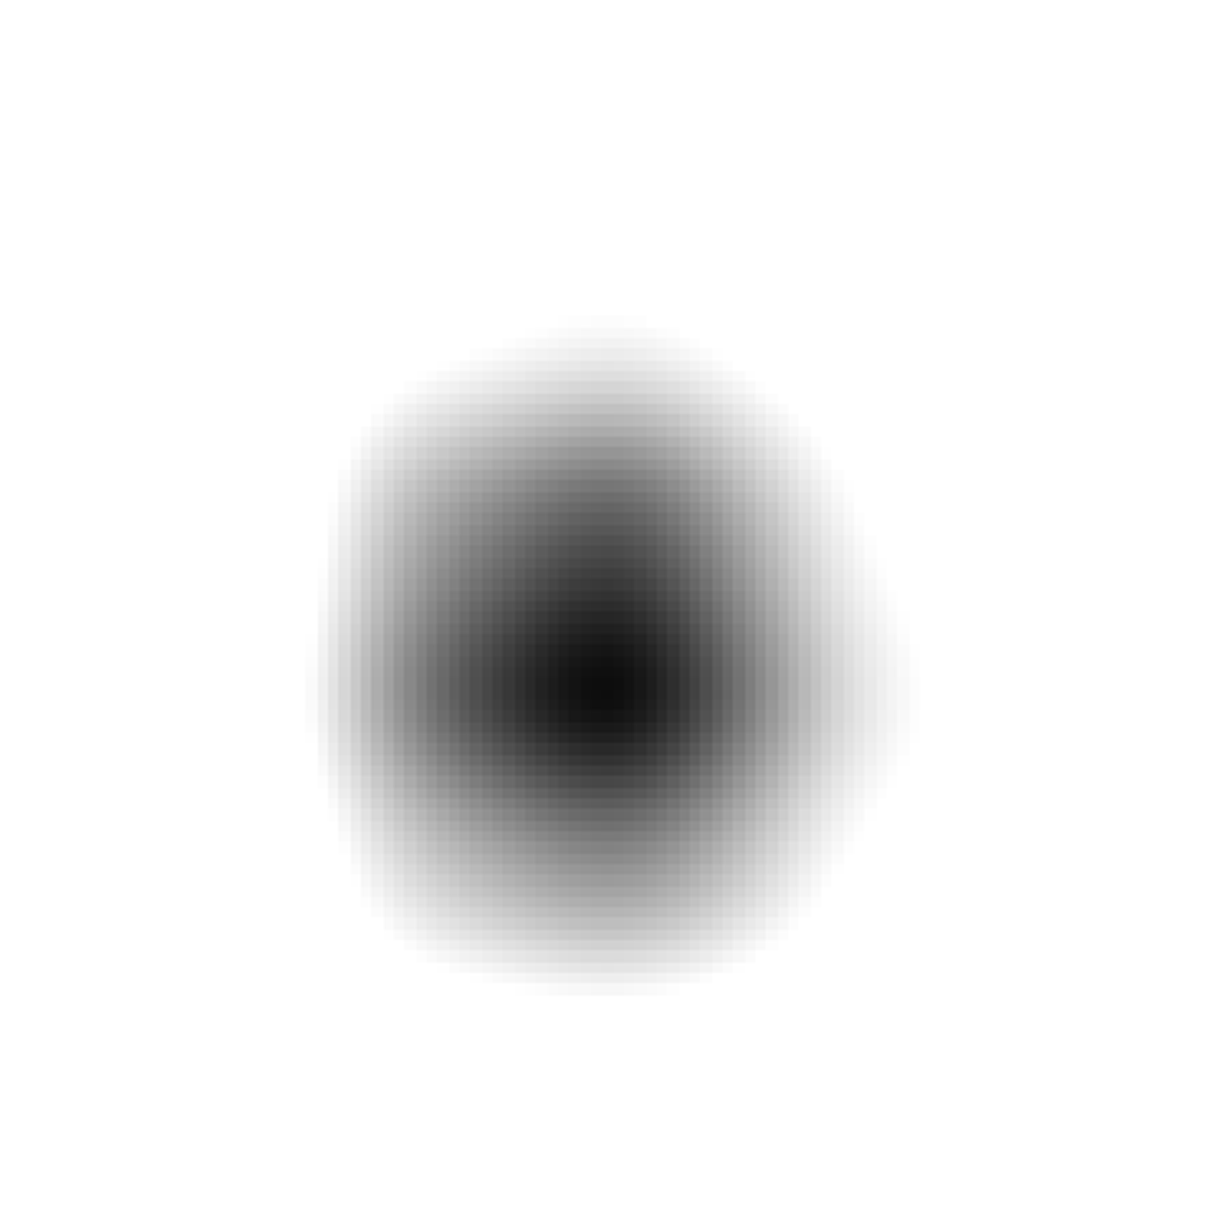
\includegraphics[scale=.11]{slicer3D/profiles/MR_x100.png}
    \caption{MRI x100}
    \label{fig:MRI_x100}
  \end{subfigure}
  \caption{CT/MRI: axial image of single rod, filling \#5  (inverted colours)}
  \label{fig:resample}
\end{figure}
\clearpage



\subsection{Capabilities}

The developed software tool is not able to automatically detect individual rods shown in a CT or MRI scan.
Instead the acquired 3D images have to be cropped to depict only a single rod.

The python script can:
\begin{itemize}
 \item denoise the image data
 \item find the brightness values of the rod, enabling it to
 \item separate pixels representing the rod from surrounding air (masking)
 \item calculate the centroid coordinates along the rod, used to
 \item calculate the local distortion
  \subitem loaction shift
  \subitem dice coefficient (roundness/deformation)
 \item plot individual rod slices
  \subitem overlaying one or two centroid coordinates
  \subitem and save it as ``.png'' file
 \item change the pixel values to reflect the distortion occuring along a rod (visualization)
 \item write the calculated numbers to a ``.txt'' file
\end{itemize}

\subsection{Measuring distortion}

Two phenomena were chosen to reflect the amount of distortion occurring in MRI scans:

\begin{enumerate}[label=\textbf{\arabic*)}]
 \item location shift (``warp'')
 \item deformation (deviation from circular profile ``DC'')
\end{enumerate}

Since the rods have a cylindrical shape, distortion can only be assessed in radial direction. To make calculations easier, the z-coordinate was put parallel to the rods, x and y radial.
Each slice (z = const.) should idealy depict the bright circular profile of the liquid (+ plastic rod in CT) surrounded by black (air).
To calculate the location shift between rods shown in CT and MRI, the coordinates of the center of mass (COM) were subtracted.
The location difference in each slice is saved as an array. Additionally, the absolute value of the coordinate shift (absCS) could be calculated.

% image of COM shift

The dice-coefficient ``DC'' (also known as Sorensen-Index) was chosen as indicator for the deviation from a circular profile. Again this value was calculated for every slice using either the CT or MRI scans.

To get a idea of the occuring distortion one should look at both the absolute value of coordinate shift and the dice-coefficient (DC).
The DC ranges from 0 to 1. A value of 1 indicates a perfect circular shape. A low DC on the other hand could be caused by many things such as:
little overlap (e.g. a ring or crescent shape); a very dark image hindering delineation of rod from background; a small circle with a radius close to a only a few pixels.


% A proposed third indicator combining warp magnitude and the DC:
% $warpDC = warpMagnitude * (1-DC)$

\subsection{Calculation: dice-coefficient (DC)}

The dice coefficient or Sorensen index \cite{MedPy_dc-doc} is defined as:

\begin{align}
DC = \frac{2 |A \, \cap \, B|}{|A| + |B|}
% what application used to align CT and MRI
\end{align}

The implementation into python is based on the open source python package ``Medpy''. \cite{MedPy} A part of it's module called ``metric'' was adapted. \cite{MedPy_dc-code}
All pixels above a certain threshold will be counted as input A. The reference B is a circle whose midpoint is placed at the COM.

The caluclation of the DC is done by comparing an binary image to a circle. The position of the circle's centre and its radius is highly influencing the outcome.
Both the circle's centre and its radius were varied during the distortion assesment.


\subsection{Calculation: center of mass (COM)}

The calculation of the COM is done with help of the ``scipy'' python package.
It's module ``ndimage'' contains the function ``$center\_of\_mass()$'', which returns the COM's coordinates of a given input array.
The values assigned to voxels in CT images lie in the range from -1024 HU (air) to around 200 HU (plastic rod).
Before a meaningful result can be obtained, the values need to be shifted to be $>$ 0.
Additionally, only pixels representing the rod or the liquid should be used for the calculation.
Otherwise the almost black voxels surrounding the rod would influence the result.
This error could be observed especially if the rod is not placed in the exact middle of the scan.
As described earlier, the plastic rod is only visible in CT images. On the MRI scanns solely the liquid containded in the rods is shown. Therefore rods appear to be smaller on the MRI data.
To find the relevant pixels two algorithms were developed:

\begin{description}
 \item[1] calculating the number of pixels based on rod size
 \item[2] finding a COM resulting in good DC
\end{description}

add 1:
The inner ($4mm$) and outer ($8mm$) diameter of the rods are known. So is the \textit{pixel spacing} which respresents the equivalent size of a voxel in $mm$.
Calculating the number of pixels which make up the more or less circular profile ot the rod in each slice is calculated like this:

\begin{align}
 pixelNumber = (radius^2 \cdot \pi) \, / \, (spacing^2)
\end{align}

For CT images $radius = 4mm$, in MRI scans $radius = 2mm$. $spacing$ is the pixel spacing in x and y direction.
Next the pixels are sorted by brigthness. The top $pixelNumber$ pixels are then used to calculate the COM.

add 2:
This algorithm is a iteration method. It starts by assuming $\approx 50\%$ of all pixels in the image are part of the rod.
This first guess of $50\%$ is shifted by multiplying it with $(1 \pm 0.2) \rightarrow 1.2$ and $0.8$.
So in the first step two possible COMs are obtained using the brightest $50*1.2 = 60\%$ and $50*0.8 = 40\%$ of all pixels.
It takes note of the values assigned to the darkest and brightest pixels used during both calculations.
Those values are then set as threshold for the DC coefficient.
Effectivly it finds COM and DC for $52\%$ and $60\%$. If the DC for using 52\% is bigger, it chooses $(100\% + 50\%) / 2 = 75\%$ as next guess.
If on the other hand the DC for $40\%$ is bigger, it chooses $(0\% + 50\%) / 2 = 25\%$ as next guess.
In the second iteration it now again shifts the percentage by multiplying it with $1.2$ and $0.8$. Again COM and DC are calculated and the next guess is chosen by comparing the DCs.
This is continued until the DC value decreases compared to DC found in prior steps. The maximum DC is used as indicator for the best COM.

% image of COM shift

\chapter{Results}
% o Present all results here
% o No discussion, no interpretation, no evaluation etc.
% o Figures / Tables
%  Use wisely
%  Consult your supervisor about what to present
%  put very large and detailed tables rather in the appendix
%  put source code in appendix
% o Do not write down all data from table in text, but put them in relation to each other
% o Help reader to understand tables & graphs and highlight important and/or interesting data
% o Present an assessment of uncertainties

On the second day of working with the filled rods the one containing liquid \textbf{\#6} broke (leakage).
It happened when delicately knocking it against on the table while standing upright.
This was intended to mobilise bubbles that sticked to the wall and make them travel vertically to on end of the rod. (see tabular \ref{tab:bubbles})
The plasic stopper on the lower end came loose.
The rod containing filling \textbf{\#6} was not replaced.
Consequently, all CT and MRI images show only 16 rods.

\section{Obtained MRI and CT scans}
Figure \ref{fig:coronal} shows a coronal view of the 16 rods filled with the tested liquids.
(in figure \ref{fig:axial_MR} a plasic bottle filled with water has been placed there instead (see figure \ref{fig:axial_CT_pane}).)
 
\begin{figure}[!tbp]
  \begin{subfigure}[b]{\textwidth}
    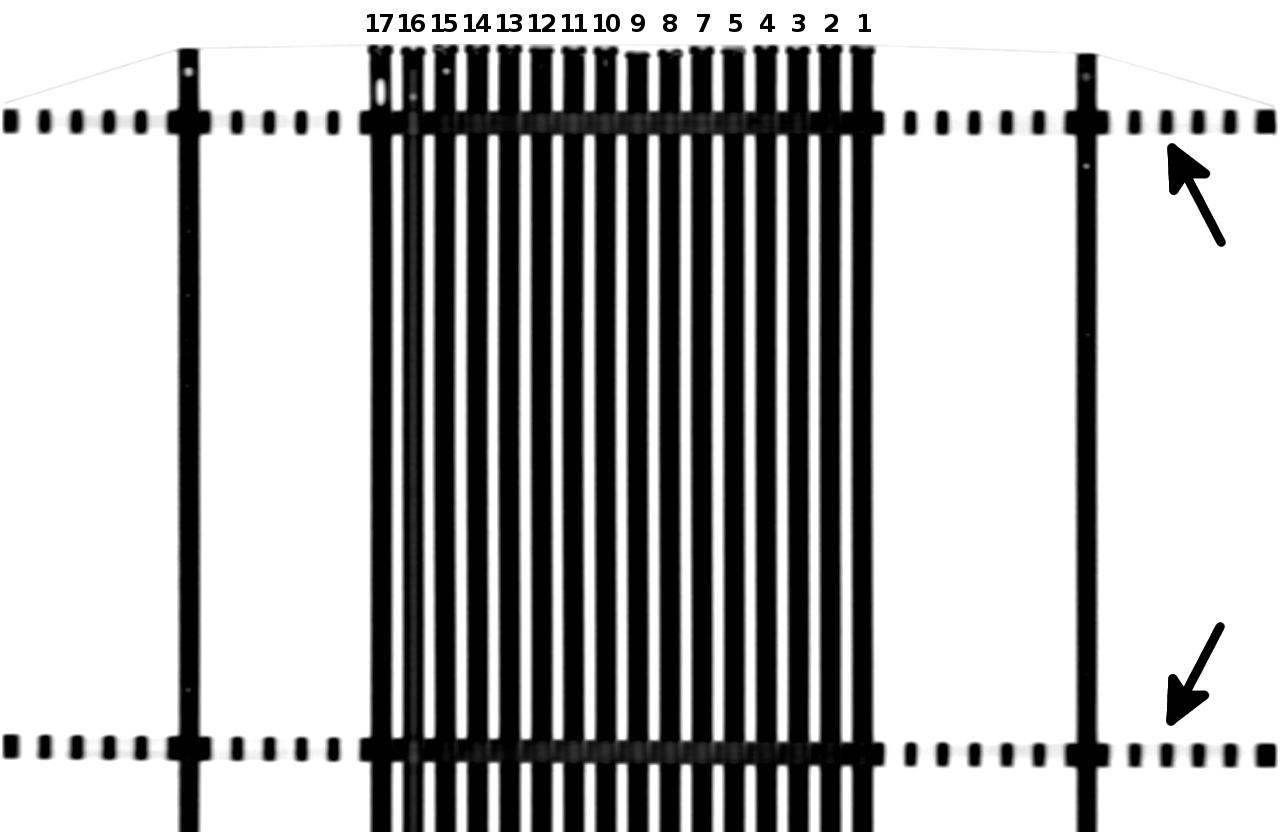
\includegraphics[width=\textwidth]{slicer3D/full_phantom/coronal_CT_cropped-arrow.png}
    \caption{CT: periodic black lines in upper and lower part of image (arrows) show plastic panes from above); rods have been fixed with adhesive tape (faint line across upper end of rods); differences in signal intensity (brightness) hardly noticeable, but air bubbles visible at upper end}
    \label{fig:coronal_CT}
  \end{subfigure}
  \begin{subfigure}[b]{1\textwidth}
    
\includegraphics[width=1\textwidth]{slicer3D/full_phantom/coronal_MR_cropped.png}
    \caption{MR: rods appear to be thinner, because only the liquid filling is visible; plastic (rods and panes) are not visible}
    \label{fig:coronal_MR}
  \end{subfigure}
  \caption{Coronal CT/MRI (inverted colours; same scale; cropped images): images of 16 rods (tested liquids, numbering starting from the right, \#6 excluded) + 2 reference rods (filled with water) on the sides; liquids result in different signal intensity (brightness)}
  \label{fig:coronal}
\end{figure}

\begin{figure}[!tbp]
  \begin{subfigure}[b]{\textwidth}
    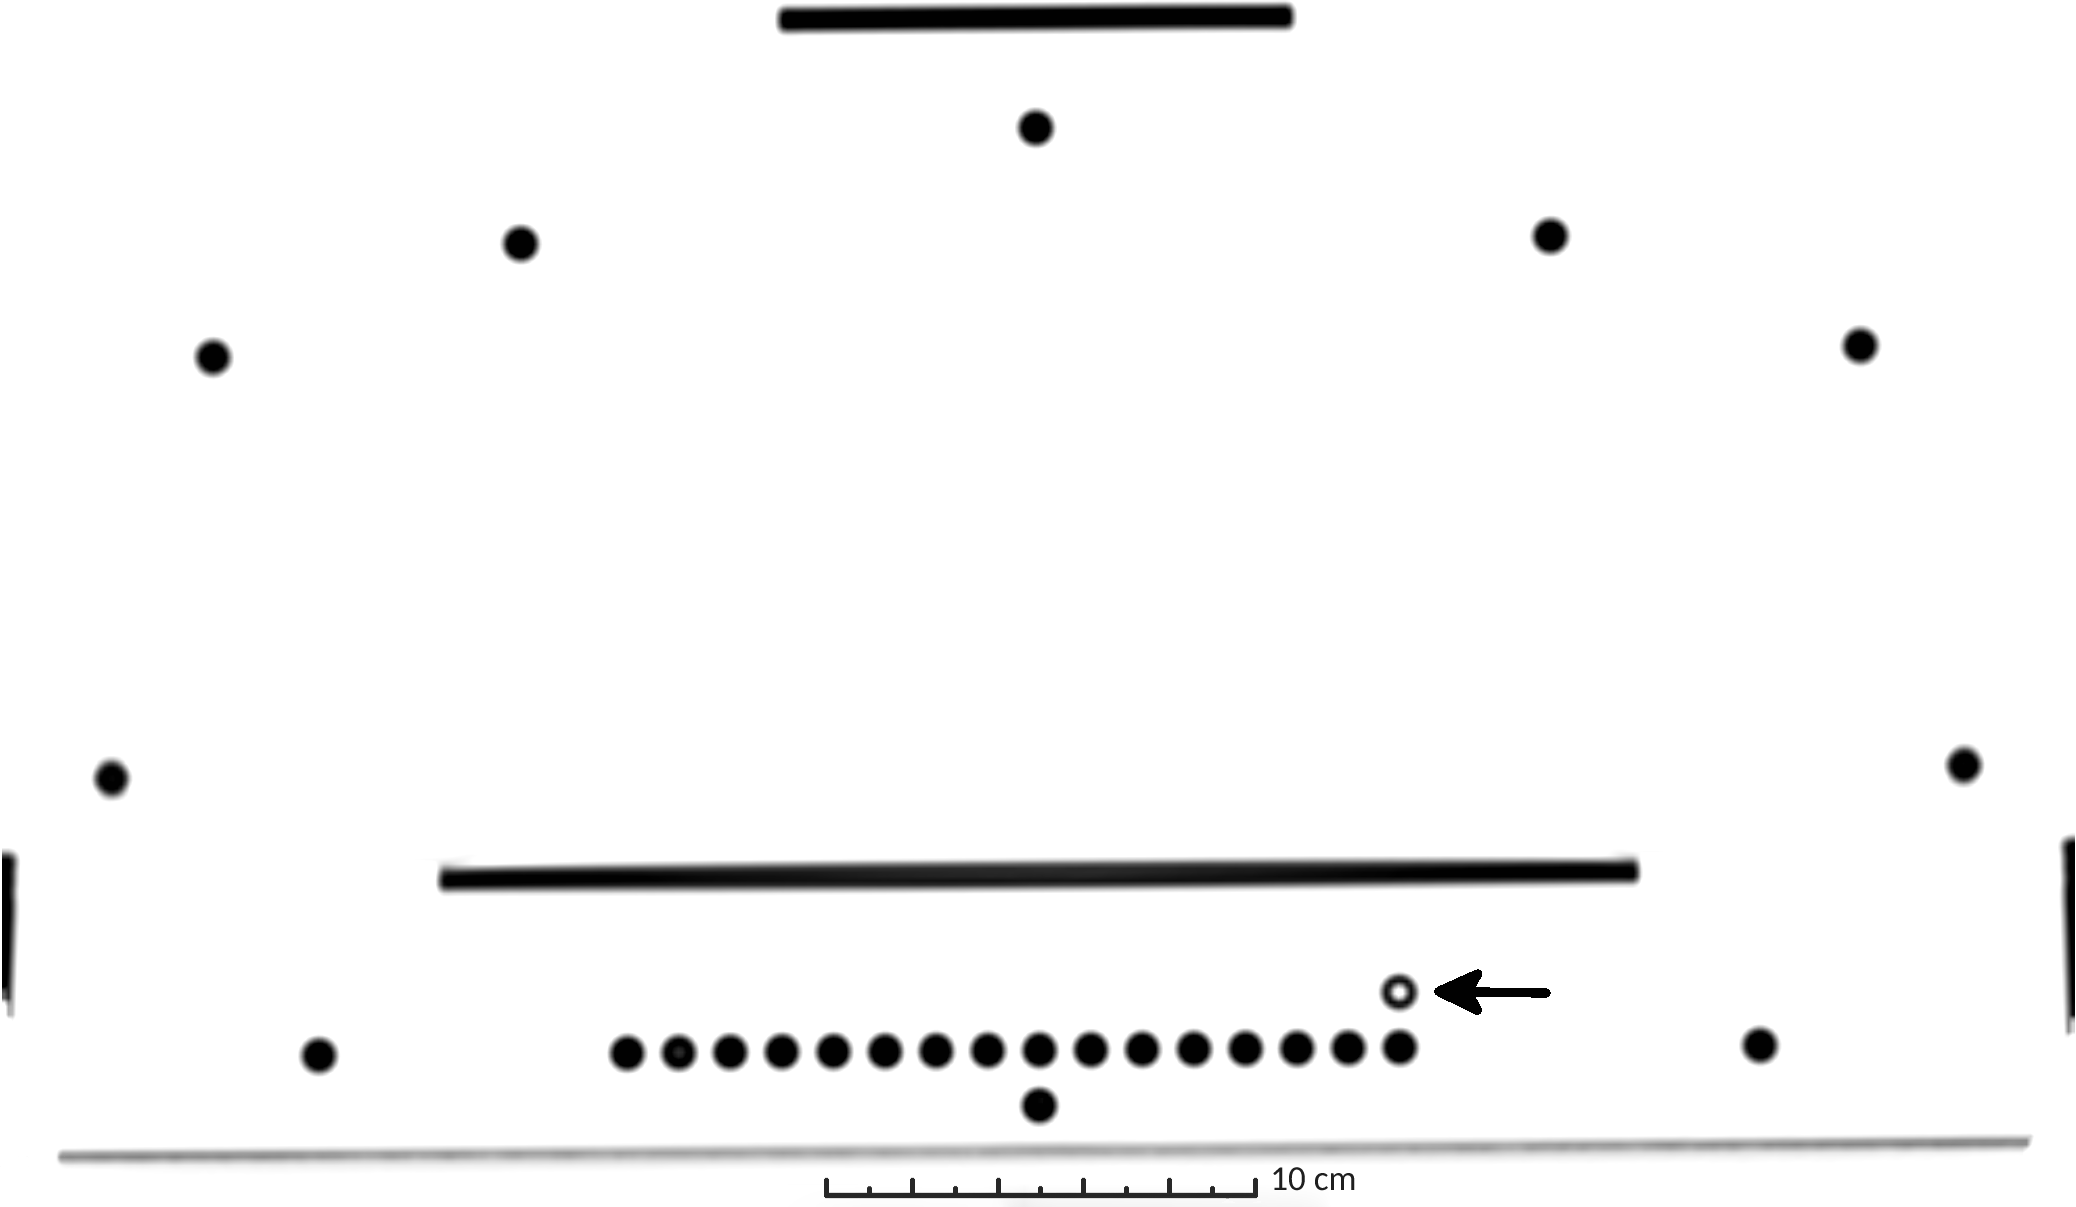
\includegraphics[width=\textwidth]{slicer3D/full_phantom/axial_CT_rods-arrow.png}
    \caption{CT: black bars just above tested rods, at the very top and to the sides show plastic parts of the phantom holding it togehter; faint grey line below tested rods shows table on which phantom was positioned during imaging}
    \label{fig:axial_CT_rods}
  \end{subfigure}
  \begin{subfigure}[b]{\textwidth}
    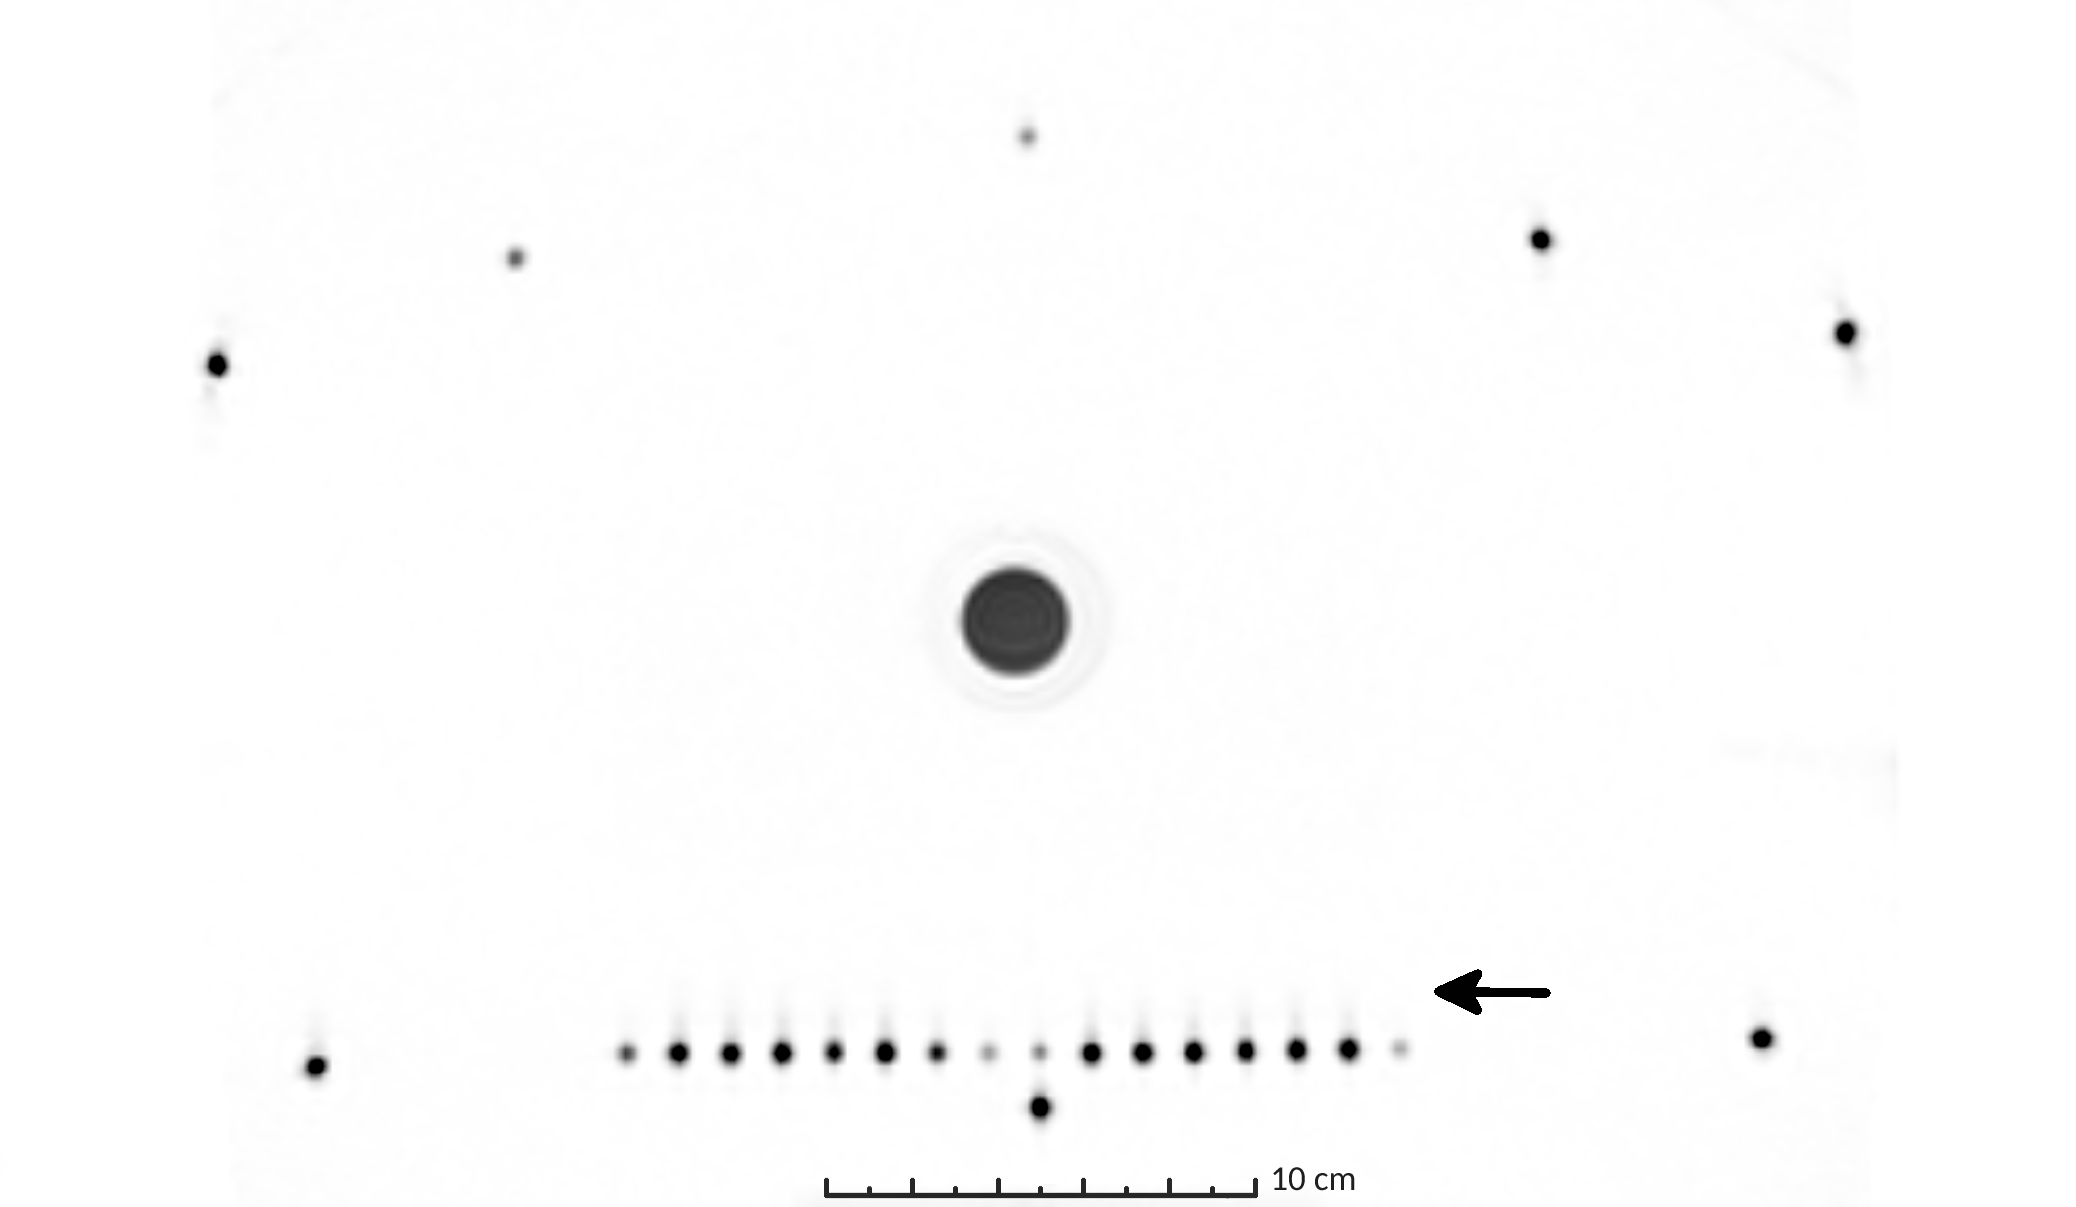
\includegraphics[width=\textwidth]{slicer3D/full_phantom/axial_MR-arrow.png}
    \caption{MRI: black circle in middle shows water bottle which was placed in the middle of the phantom (necessary for MRI scanner to start imaging)}
    \label{fig:axial_MR}
  \end{subfigure}
  \caption{axial CT/MRI (inverted colours, same scale): images of 16 rods (tested liquids, numbering starting from the right, \#6 excluded); surrounded by reference rods (filled with water) and one empty rod (marked with arrow) which is not visible on MRI scans}
  \label{fig:axial}
\end{figure}


\section{Tested solutions}

\subsection{Visibility on CT/MRI scans}

Generally, imaging techniques aims for a high signal-to-noise ratio.
Therefore, Liquids resulting in brighter pixels are favoured.

CT images show little differences between the tested liquids. The plasic rods themselves result in brigher pixels than any of the tested solutions.

On MRI scans most liquids had a mean and a max brightness value above $1000$ (see table \ref{tab:visibility}).\\
Only \textbf{\#1}, \textbf{\#9}, \textbf{\#10}, \& \textbf{\#17} resulted in significantly less signal.


\begin{table}[]
\centering
\begin{tabular}{@{}lllllllr@{}}
\toprule
Nr. & Min  & Max  & Mean   & Median & RMS    & $\sigma$     & Volume [$mm$] \\ \midrule
1   & 182  & 371  & 288    & 269    & 296,3  & 69,8  & 48.8 \\
2   & 1044 & 1921 & 1443,8 & 1405   & 1477,3 & 312,9 & 39.1 \\
3   & 941  & 2075 & 1451,2 & 1394,5 & 1508,9 & 413,2 & 39.1 \\
4   & 1176 & 1709 & 1440   & 1437,5 & 1458,6 & 232,5 & 39.1 \\
5   & 1125 & 2111 & 1583,8 & 1549,5 & 1623   & 355   & 39.1 \\
7   & 971  & 2241 & 1466,8 & 1316   & 1540,6 & 471,2 & 48.8 \\
8   & 1459 & 1947 & 1704   & 1705   & 1713,5 & 180,5 & 39.1 \\
9   & 385  & 584  & 486,8  & 489    & 495,6  & 93    & 39.1 \\
10  & 247  & 502  & 343,6  & 266    & 361,1  & 111   & 48.8 \\
11  & 830  & 1268 & 1036,2 & 1023,5 & 1049   & 163,2 & 39.1 \\
12  & 1158 & 2211 & 1648,8 & 1613   & 1695,2 & 394,2 & 39.1 \\
13  & 836  & 1657 & 1146,8 & 1047   & 1190,9 & 321,2 & 39.1 \\
14  & 800  & 2062 & 1383   & 1335   & 1461,7 & 473,1 & 39.1 \\
15  & 1156 & 1829 & 1476,2 & 1460   & 1501,2 & 272,7 & 39.1 \\
16  & 1102 & 1967 & 1509   & 1483,5 & 1543,8 & 325,8 & 39.1 \\
17  & 356  & 938  & 629,6  & 602    & 668,1  & 223,6 & 48.8 \\ \bottomrule
\end{tabular}
\caption{liquid visibility on MRI scan}
\label{tab:visibility}
\end{table}

% 
% \begin{table}[]
% \centering
% \begin{tabular}{@{}l|rrr@{}}
% Nr.	& brightest MRI pixel	& darkest CT pixel [$HU$]	& CT @ brightest pixel MRI	\\
% \toprule
% \#1	& 342			& -6		& 7		\\
% \#2	& 1777			& 31		& 31		\\
% \#3	& 1771		& 5		& 8			\\
% \#4	& 1589		& 62		& 62			\\
% \#5	& 1691		& -6		& -2			\\
% \#6	&  \multicolumn{3}{c}{\textit{------------------------ rod was leaking ---------------------------}}	\\
% \#7	& 1725		& 7		& 20			\\
% \#8	& 1868		& -40		& 43			\\
% \#9	& 514		& -11		& -11			\\
% \#10	& 477		& 1		& 1			\\
% \#11	& 1246		& -12		& 7			\\
% \#12	& 1794		& 18		& 18			\\
% \#13	& 1416		& 152		& 157			\\
% \#14	& 1814		& 4		& 4			\\
% \#15	& 1705		& 11		& 32			\\
% \midrule
% \#16	& 1848		& -196		& -196			\\
% \#17	& 836 		& 123		& 129			\\
% \bottomrule
% \end{tabular}
% \caption{liquid visibility}
% \label{tab:visibility}
% \end{table}

\subsection{Mechanical properties of solutions}
A suitable filling would yield good image contrast in CT and MRI and acceptable mechanical properties.

The liquids were filled in a rod each and observed for several months. Some solutions produced air bubbles, which would eventually lead to incorrect calculations.
Each rod was free of bubbles after sealing. The amount of gas inside the rods was measured after 2 months. Ideally, tilting the entire phantom slightly should be enough to fix all rods in the phantom at the same time.
In some of the tested rods the produced air bubbles would stick to the wall. Only after gently hitting the rod they would start moving (see table \ref{tab:bubbles}).

\begin{table}[]
\centering
\begin{tabular}{l|lc|lc|lc}
    & \multicolumn{2}{c}{\textit{after 1 day}} 	& \multicolumn{2}{c}{\textit{after 2 days}}	& \multicolumn{2}{c}{\textit{after 1 week}}	\\ 
Nr. & bubbles	& hit req.	& bubbles 	& hit req.	& bubbles 	& hit req.	\\
\toprule
\#1   & yes	& no		& no		&		& no		&		\\
\#2   & yes	& yes		& no		&		& no		&		\\
\#3   & yes	& yes		& no		&		& no		&		\\
\#4   & yes	& yes		& no		&		& no		&		\\
\#5   & yes	& no		& yes		& no		& no		&		\\
\#6   & yes	& no		& \multicolumn{4}{l}{-----------------\textit{ rod was leaking }------------------}	\\
\#7   & yes	& no		& yes		& no		& yes		& no		\\
\#8   & no	&		& no		&		& no		&		\\
\#9   & no	&		& no		&		& no		&		\\
\#10  & no$^1$	&		& yes		& yes		& yes		& yes		\\
\#11  & no	&		& yes,		& \textit{sticked to wall} &	 yes	& yes\\
\#12  & yes	& yes		& yes,		& \textit{sticked to wall} &	 yes	& yes\\
\#13  & yes	& yes		& yes,		& \textit{sticked to wall} &	 yes	& yes\\
\#14  & no	&   		& yes		& no		& yes		& yes		\\
\#15  & no	&   		& no		&		& no		&		\\
\#16  & no	&   		& no		&		& no		&		\\
\#17  & no	&   		& no		&		& no		&		\\
\bottomrule
\end{tabular}
\begin{tabular}{l|lr}
\multicolumn{3}{c}{}								\\
& \multicolumn{2}{c}{\textit{after 2 months}}					\\ 
Nr. & lenght of trapped bubble $l$ [$mm$] 	& approx. volume $V$ [$mm^3$]	\\
\toprule
\#1   & 2					& 25.13				\\
\#2   & 1.8					& 22.62				\\
\#3   & 1+1 (air blockage, at lower end)	& 25.13				\\
\#4   & 4					& 50.27				\\
\#5   & 1.5 (many small bubbles)		& 18.85				\\
\#6   & \multicolumn{2}{c}{-----------------------------\textit{ rod was leaking }------------------------------}\\
\#7   & 2 (many small bubbles)			& 25.13				\\
\#8   & 2.3					& 28.90				\\
\#9   & 3					& 37.70				\\
\#10  & 2.4					& 30.16				\\
\#11  & 2					& 25.13				\\
\#12  & 2					& 25.13				\\
\#13  & 2.3					& 28.90				\\
\#14  & 1.5+0.5 (big imobile bubble, at center)	& 25.13				\\
\#15  & 3.4 (agar gel dried)			& 42.73				\\
\#16  & 0					& 0.00				\\
\#17  & 0.5					& 6.28				\\
\bottomrule
\end{tabular}
\caption{solutions, observations}
\label{tab:bubbles}
\end{table}

Knowing the inner diameter $d$ of the rods we can easily approximate the volume of gas trapped:

\begin{align}
 V = \frac{d^2}{4}\cdot \pi \cdot l
\end{align}

% \begin{table}[p]
%   \centering
%   \rotatebox{90}{
%     \begin{minipage}{\textheight}\footnotesize
%       \centering
%       \begin{tabular}{@{}r|cccc|ccccrrr@{}}
% 	    & \multicolumn{4}{c}{\textit{after 1 day}}	& \multicolumn{4}{c}{\textit{after 2 days}}			& \multicolumn{4}{c}{\textit{after 1 week}}&		 \multicolumn{4}{c}{\textit{after 2 months}}                 \\ 
% 	    & \multicolumn{4}{c}{} 			& \multicolumn{4}{c}{}                             \\
% 	Nr. & bubbles	& angle		& hit req.	& bubbles 	& angle		& hit req.	&  \\
% 	\toprule
% 	1   & yes	& $10^o$	& no		& no		&		&		&   \\
% 	2   & yes	& $40^o$	& yes		& no		&		&		&   \\
% 	3   & yes	& $40^o$	& yes		& no		&		&		&   \\
% 	4   & yes	& $80^o$	& yes		& no		&		&		&   \\
% 	5   & yes	& $10^o$	& no		& yes		& $10^o$	& no		&   \\
% 	6   & yes	& $10^o$	& no		& \multicolumn{5}{r}{--------------\textit{ rod was leaking }------------} \\
% 	7   & yes	& $10^o$	& no		& yes		& $10^o$	& no		&   \\
% 	8   & no	&		&   		& no		&		&		&   \\
% 	9   & no	&		&   		& no		&		&		&   \\
% 	10  & no$^1$	&		&   		& yes		& $20^o$	& yes		&   \\
% 	11  & no	&		& yes		& yes		& \multicolumn{4}{r}{---\textit{ bubbles sticked to wall }---} \\
% 	12  & yes	& $60^o$	& yes		& yes		& \multicolumn{4}{r}{---\textit{ bubbles sticked to wall }---} \\
% 	13  & yes	& $80^o$	& yes		& yes		& \multicolumn{4}{r}{---\textit{ bubbles sticked to wall }---} \\
% 	14  & no	&		&   		& yes		& $40^o$	& no		&   \\
% 	15  & no	&		&   		& no		&		&		&   \\
% 	16  & no	&		&   		& no		&		&		&   \\
% 	17  & no	&		&   		& no		&		&		&   \\
% 	\bottomrule
%       \end{tabular}
%       \caption{Messwerte}
%       \label{tab:wirkungsgrad}
%     \end{minipage}
%   }
% \end{table}

\section{Distortion assesment}
All results were obtained by manually cropping the 3D image to depict only a single rod.
\subsection{Distortion}

\vspace{4cm}
\textit{table showing distrortion along z axis (isocentre to image border)}
\vspace{2cm}

\begin{figure}[!tbp]
  \begin{subfigure}[b]{0.32\textwidth}
    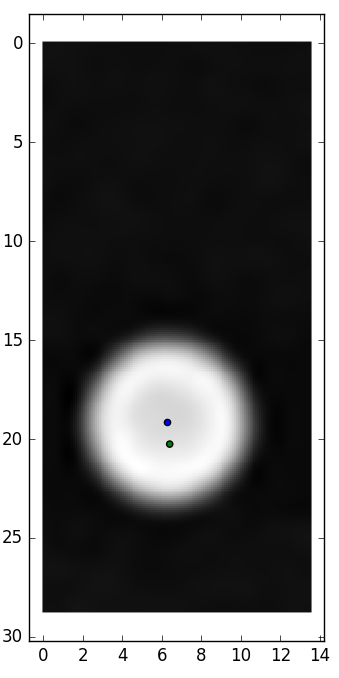
\includegraphics[scale=0.55]{python/centroid/CT_x100@0_centroids.png}
    \caption{CT @ 0}
    \label{fig:CT_x100_centroids@0}
  \end{subfigure}
  \begin{subfigure}[b]{0.32\textwidth}
    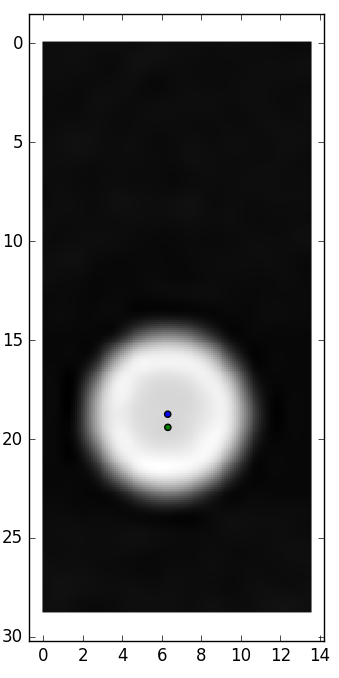
\includegraphics[scale=0.55]{python/centroid/CT_x100@150_centroids.png}
    \caption{CT @ 150}
    \label{fig:CT_x100_centroids@150}
  \end{subfigure}
  \begin{subfigure}[b]{0.32\textwidth}
    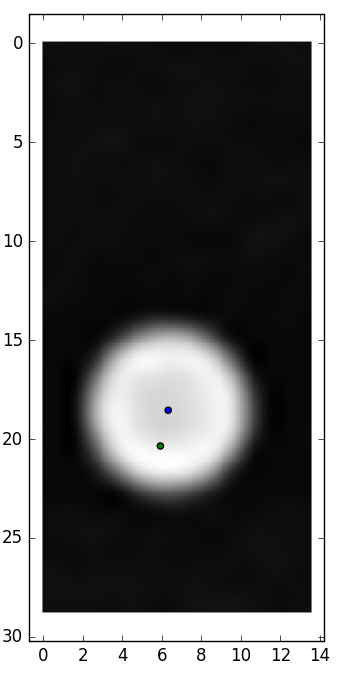
\includegraphics[scale=0.55]{python/centroid/CT_x100@304_centroids.png}
    \caption{CT @ 304}
    \label{fig:CT_x100_centroids@304}
  \end{subfigure}
  \begin{subfigure}[b]{0.32\textwidth}
    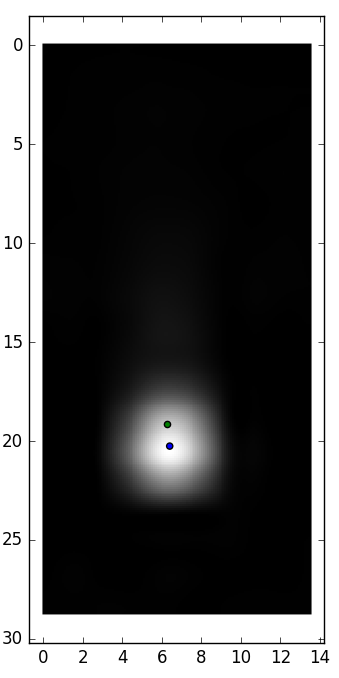
\includegraphics[scale=0.55]{python/centroid/MR_x100@0_centroids.png}
    \caption{MRI @ 0}
    \label{fig:MR_x100_centroids@0}
  \end{subfigure}
  \begin{subfigure}[b]{0.32\textwidth}
    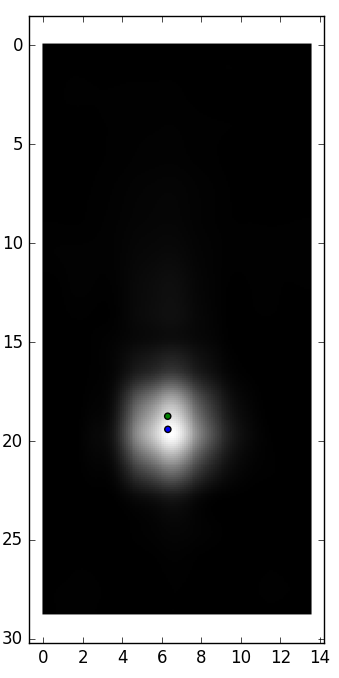
\includegraphics[scale=0.55]{python/centroid/MR_x100@150_centroids.png}
    \caption{MRI @ 150}
    \label{fig:MR_x100_centroids@150}
  \end{subfigure}
  \begin{subfigure}[b]{0.32\textwidth}
    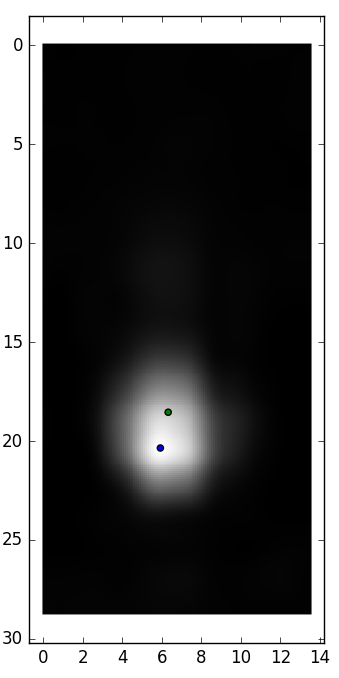
\includegraphics[scale=0.55]{python/centroid/MR_x100@304_centroids.png}
    \caption{MRI @ 304}
    \label{fig:MR_x100_centroids@304}
  \end{subfigure}
  \caption{MRI x100; blue dot centroid MRI, green dot centroid CT (same scale);\\ slice 150 is approximately at the isocentre, 0 on the very end of the image, 304 close to an air bubble}
  \label{fig:MR_x100_centroids}
\end{figure}

\vspace{2cm}

\subsection{DC}


\begin{figure}[!bp]
  \centering
  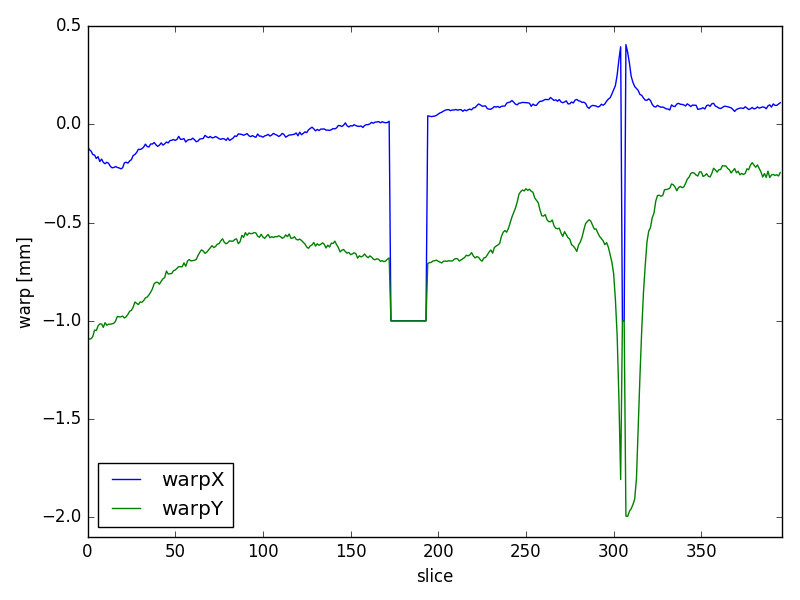
\includegraphics[scale=0.65]{python/warp/warpXY_x100--.png}
  \caption{warp XY [$mm$], CT-MRI x100}
  \label{fig:warpXY_x100}
\end{figure}

\newpage

\begin{figure}[!tp]
    \centering
    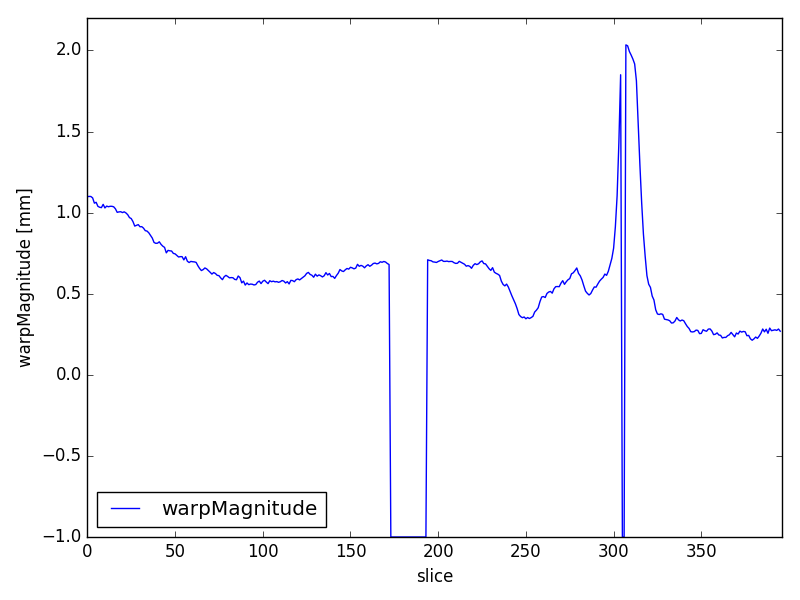
\includegraphics[scale=0.65]{python/warp/warpMagnitude_x100--.png}
    \caption{warp Magnitude [$mm$], CT-MRI x100}
    \label{fig:warpMagnitude_x100}
\end{figure}
\begin{figure}[!bp]
    \centering
    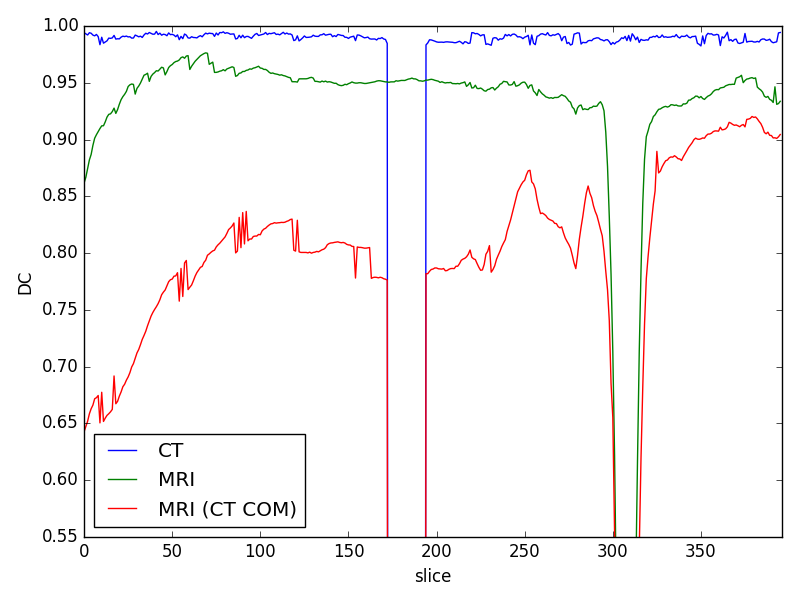
\includegraphics[scale=0.65]{python/dice/CT_MR_x100_DC.png}
    \caption{DC (optimised) for CT \& MRI \& MRI (using CT COM)}
    \label{fig:CT_MR_x100_DC}
\end{figure}

\begin{figure}[!bp]
    \centering
    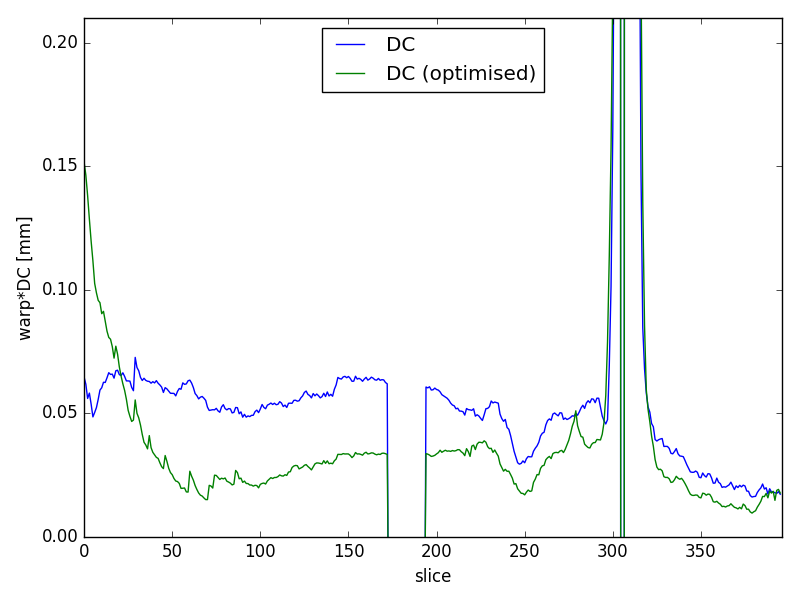
\includegraphics[scale=0.65]{python/warpDC/warpDC_x100.png}
    \caption{artificial indicator warp*DC using real DC and optimised DC of MRI x100}
    \label{fig:warpDC_x100}
\end{figure}
\begin{figure}[!bp]
  \centering
  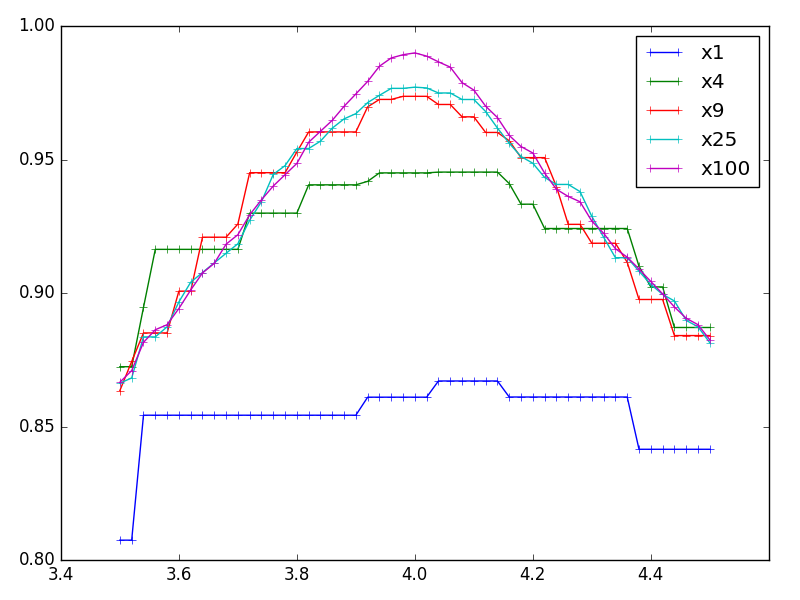
\includegraphics[scale=0.65]{python/dice/CT-51iter.png}
  \caption{CT: DC of varied radii \& resolutions}
  \label{fig:CT_dc}
\end{figure}

\begin{figure}[!tbp]
  \begin{subfigure}[b]{\textwidth}
    \centering
    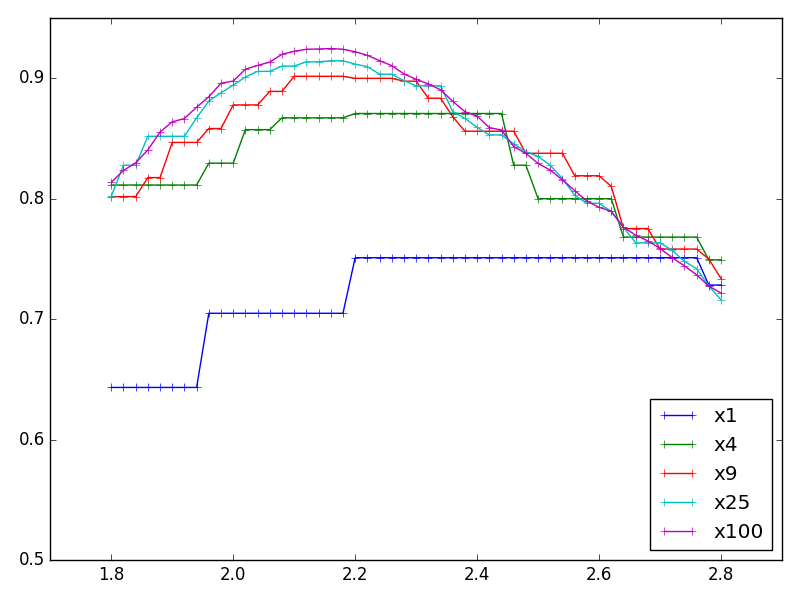
\includegraphics[scale=0.65]{python/dice/MR-51iter.png}
    \caption{MRI: DC of varied radii \& resolutions}
    \label{fig:MR_dc-opti}
  \end{subfigure}
  \begin{subfigure}[b]{\textwidth}
    \centering
    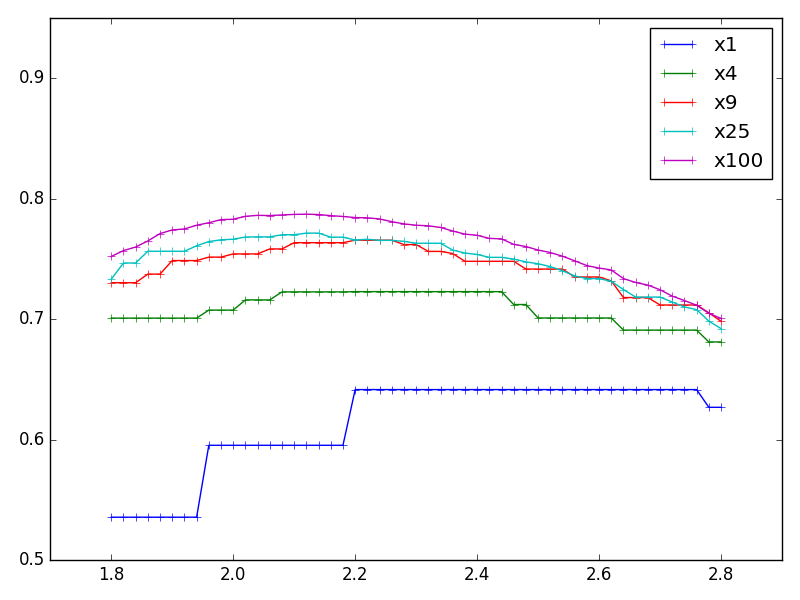
\includegraphics[scale=0.65]{python/dice/MR_CT-COM_51iter.png}
    \caption{MRI: DC of varied radii \& resolutions (using CT-COM)}
    \label{fig:MR_CT-COM_dc-opti}
  \end{subfigure}
  \caption{}
  \label{fig:MR_dc}
\end{figure}


The obtained dice coefficient varies not only because of the circle's centre and the radius, it also depends on the images resolution.
Figure \ref{fig:CT_dc} and \ref{fig:MR_dc} show the DC (optimised) obtained using CT and MRI scans over resample rate.

% \begin{figure}[!tbp]
%   \begin{subfigure}[b]{\textwidth}
%     \centering
%     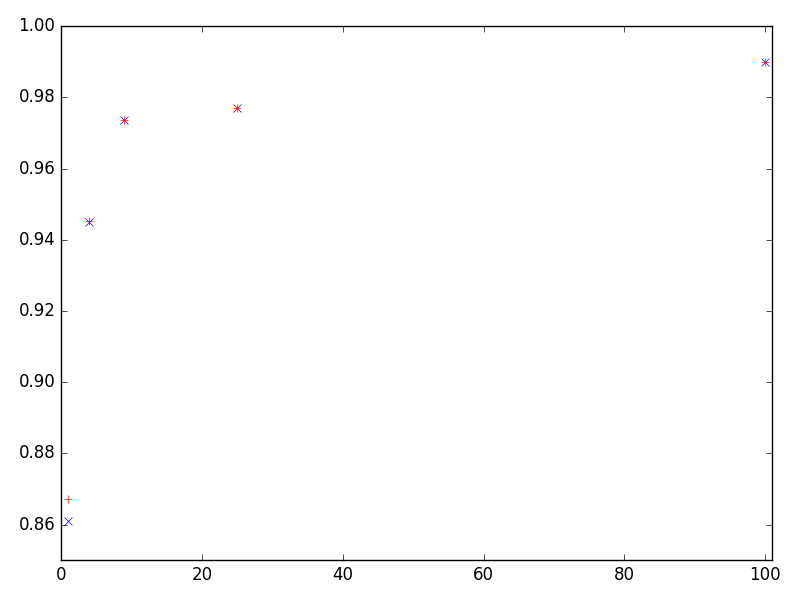
\includegraphics[scale=0.65]{python/dice/CT_dice-comparison_fast-51iter.png}
%     \caption{CT: x1, x4, x9, x16, x25, x100}
%     \label{fig:MR_dice-comp}
%   \end{subfigure}
%   \begin{subfigure}[b]{\textwidth}
%     \centering
%     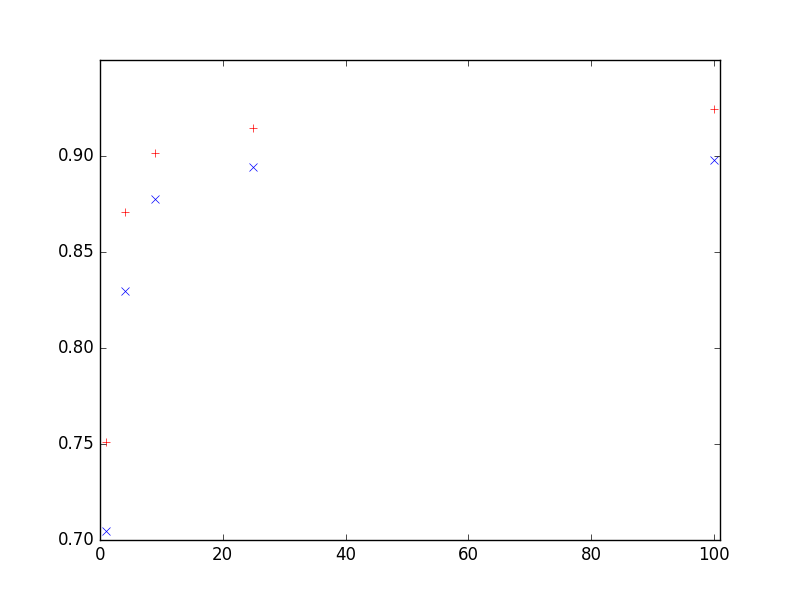
\includegraphics[scale=0.65]{python/dice/MR_dice-comparison_fast-51iter.png}
%     \caption{MRI: x1, x4, x9, x16, x25, x100}
%     \label{fig:MR_dice_comp}
%   \end{subfigure}
%   \caption{}
%   \label{fig:dice_com}
% \end{figure}

% image of COM shift
\chapter{Discussion}
% o Interpretation of results, putting them in context with literature
% o Discuss only results which were presented in the results section and do not repeat them one by one
% o Which impacts have your results on the scientific community?
% o provide an assessment of the weaknesses and strengths of your work
% o At least 5 pages


\section{Tested solutions}

For measuring the position of the rods in the CT scans the plastic rods without filling would be enough already, they would not be visible on the MRI scans, though.

Oil generally shows good visibility in CT and MRI scanns and produces no air bubbles after closing.
However, filling all rods of the phantom with Oil is considered the last option. Water based liquids prove to be easier to clean.
Since topping up over 300 rods regularily is too time consuming, oil seems to be a good alternative.
However, if air bubbles could be easily shifted towards one end of the rod by tilting it slightly, they would lie outside the MRI scanner's field of view.
Consequently, it would be sufficient to move air bubbles to one end of the rod before imaging.


\section{Distortion}
An air bubble might lead to a incorrect COM. Without looking at the dice-coefficient it's hard to tell why this distortion only appears to be present in a few slices.
If both indicators show unexpected local irregularities, a conclusion might be easier to draw.

\chapter{Conclusion and Outlook}
% o Summary of study
%  Most important results and their meaning/impact and conclusions
%  Outlook
%  open questions
%  Next steps

\section{Preparing the phantom for distortion assesment}

\section{Future improvement of software tool}

Future improvements of the developed software tool are supposed to:
\begin{itemize}
 \item find and register all individual rods automatically
 \item calculate the local distortion
 \item create a 3D vector map
\end{itemize}


\bibliography{MRI-for-RT.bib}
\bibliographystyle{ieeetr}

\end{document}


% what application used to align CT and MRI
% photo of phantom
% image of COM shift
% interpolate CT slices where plastic pane is??!?
% add slice thickness to figures (DC, Warp, etc.)
% MRI values are 
% CTNumbers = HU
% remove "Volume" Column from table with mean, max, min values of MRI rods
% add reference circle to figure showing resampled CT and MRI slices
% only 2 digits after komma in table with pixel spacing
% use examples for different DC values + images
